% CHAPTER 1
\chapter{INVESTIGATION OF INERTIAL SUPPORT PRACTICAL LIMITS}
\label{chp:4}
\section{Inertial Support Limits}
The source of power in a wind turbine is the aerodynamic wind power, $P_{wind}$ which is constant for a constant wind speed, pitch angle and generator speed. In the steady state, this power is transferred through MSC as $P_{gen}$. If there is a difference between $P_{wind}$ and $P_{gen}$, the difference is either stored in or extracted from the turbine and generator inertia as in the form of kinetic energy. Grid power, $P_{grid}$ is received from MSC and injected grid. The difference between $P_{gen}$ and $P_{grid}$ is stored in or extracted from DC-bus capacitance. The active power flow diagram is depicted in Fig. \ref{power_flow}. As mentioned in Chapter \ref{chp:3}, stored energy exists in turbine and generator inertia and DC-bus capacitance. However, it is also stated that the $E_{kin}$ is much larger than $E_{DC}$ even in the lowest generator speed. Therefore, the source of the inertial support studies is the kinetic energy stored in the inertia. \par
\begin{figure}[h!]
	\centering
	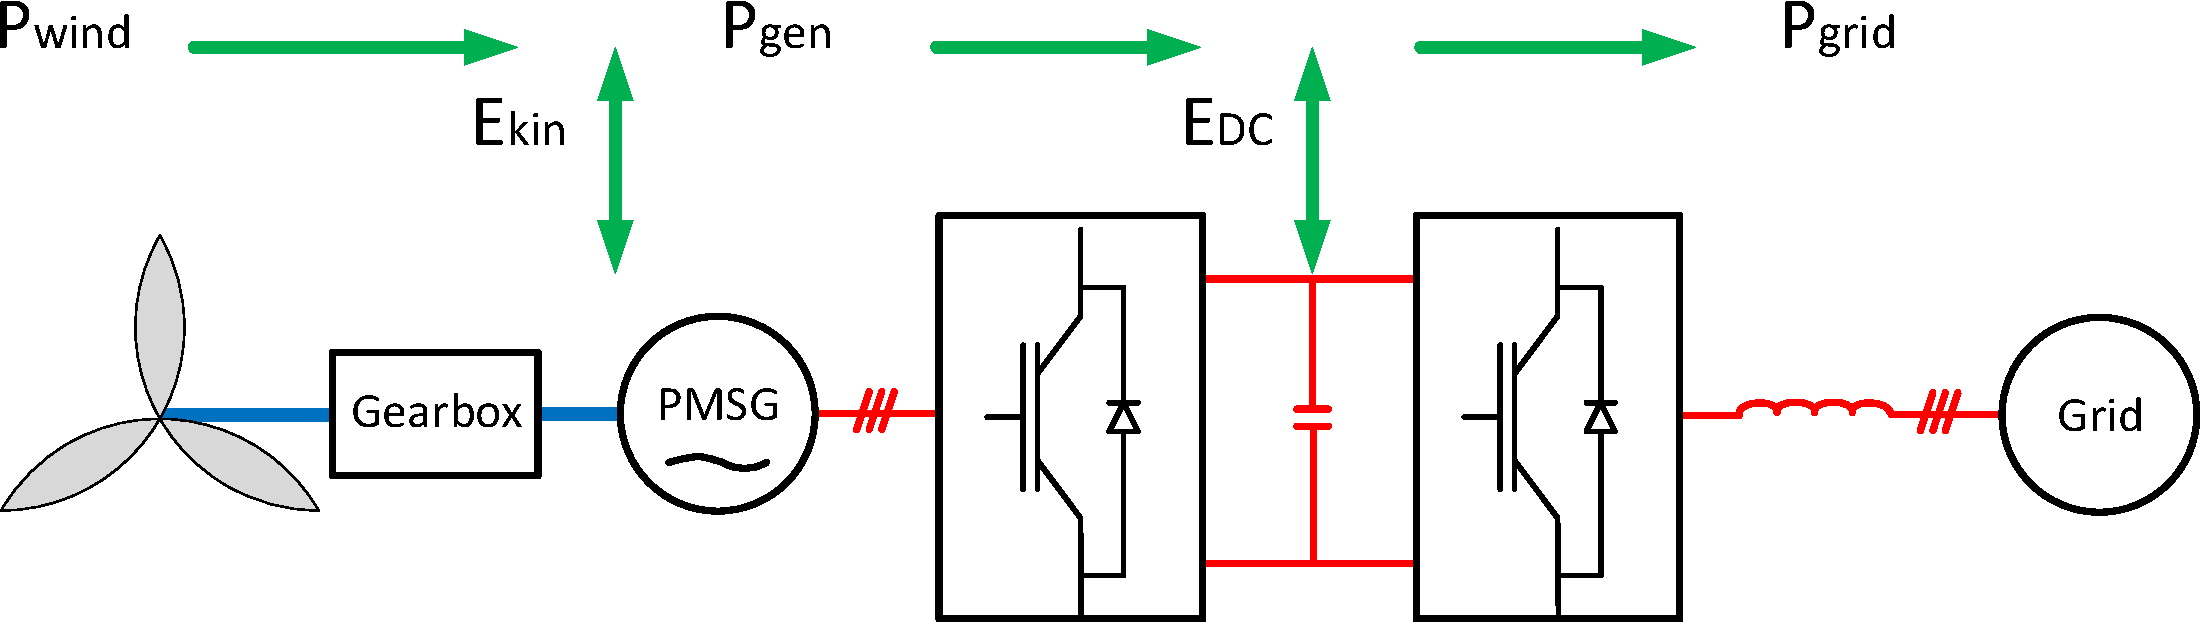
\includegraphics[width=.95\linewidth]{power_flow.pdf}
	\caption{Active Power Flow Diagram}
	\label{power_flow}
\end{figure}
Wind turbine active power can be increased by increasing the generator power $P_{gen}$. This can be achieved by adjusting the generator torque since the active power is proportional to electromagnetic torque. However, the active power is also dependent on the generator rotational speed as in Eq. (\ref{genpower}). The active power can be increased by increasing the torbine torque but the increase is limited by the generator speed. Therefore, the active power increase is also dependent on the wind speed which determines MPPT speed in the steady state.
\begin{equation}
P_{gen}=T_{e} \omega_{m}
\label{genpower}
\end{equation}
Note that the source of the additional power is the kinetic energy stored in the turbine equivalent inertia. Therefore, as soon as the power is increased, the turbine and generator speeds start decreasing. Therefore, the electromagnetic torque should be increased to keep the generator power constant. The time duration that generator power is increased and the initial generator speed will determine the final generator speed as in the Eq. (\ref{finalspeed}).
\begin{equation}
 \int_{t_{i}}^{t_{f}}P_{wind}- \int_{t_{i}}^{t_{f}}P_{gen}=\Delta E_{kin}=\frac{1}{2}J_{tur}(\omega_{f}^2-\omega_{i}^2)
\label{finalspeed}
\end{equation}
As seen from the Eq. (\ref{genpower}), the generator power is the multiplication of generator torque and speed. In the high speeds, the generator speed $\omega_{m}$, cannot be controlled with only the generator torque but also with the pitch angle. In this way, the rated power is not exceeded as in the Eq. (\ref{maxpower}) by maintaining the maximum generator speed and maximum generator torque. However, general practive is employing higher power rating converter than generator active power rating in the variable speed wind turbines. Therefore, higher limit torque can be used in such wind turbine applications by considering the apparent power of the back-to-back converters. Therefore, the maximum power for a wind speed can be defined as in Eq. (\ref{maxxpower}).
\begin{equation}
P_{rated}=T_{P-lim} \omega_{max}
\label{maxpower}
\end{equation}
\begin{equation}
P_{max}=T_{S-lim} \omega_{max}
\label{maxxpower}
\end{equation}
\section{Inertial Support Under Different Wind Speeds}
Active power of the wind turbines is determined by parameters such as wind speed, pitch angle and turbine speed. Therefore, combination of these parameters have importance for a possible inertial support. In other words, wind turbine under high wind scenario has different potential than that under low wind scenario. Likewise, the resultant states of wind turbines for inertial support would be much different. In this chapter, the effect of wind speed will be investigated for inertial support. Active power of wind turbines will be increased by different percentages. The change in generator speed, turbine and generator torques, DC-link voltage and pitch angle, if any, will be observed. Wind turbine used in this study is GE 2.75-103 model, variable speed PMSG.
\subsection{Low Wind Scenario}
\label{sec:lowwind}
The minimum speed of the wind turbine in this scenario is 550 rpm in the high speed side. Wind speed that will capture the maximum power from wind in this generator speed is found out to be 3.12m/s. In this scenario, the kinetic energy stored in the turbine inertia is minimum and calculated in Chapter \ref{chp:4} in Eq. (\ref{kineticenergymin}). This scenario investigates the case where the least amount of kinetic energy exists in the turbine equivalent inertia.\par
\subsubsection{Active Power Limit in Low Wind Scenario}
The electricity grid in the upcoming future might require sudden active power release from wind farms for short time durations. Therefore, it is important to observe the maximum achievable power for inertial support studies. The equation Eq. (\ref{maxxpower}) implies that wind turbine in the low wind speed scenario cannot reach rated active power since the generator speed is much lower than the maximum generator speed. However, the electromagnetic torque in steady state is much lower than the limit torque, $T_{S-lim}$. Therefore, the wind turbine in low speed scenario has the potential for increasing its active power to a significant value. Fig. \ref{low_limit_power} shows the increase of active power to maximum value. The increase is obtained by ensuring the limit torque, $T_{S-lim}$. However, since the generator speed is decreasing, the active power is also decreasing. 

\begin{figure}[h!]
	\centering
	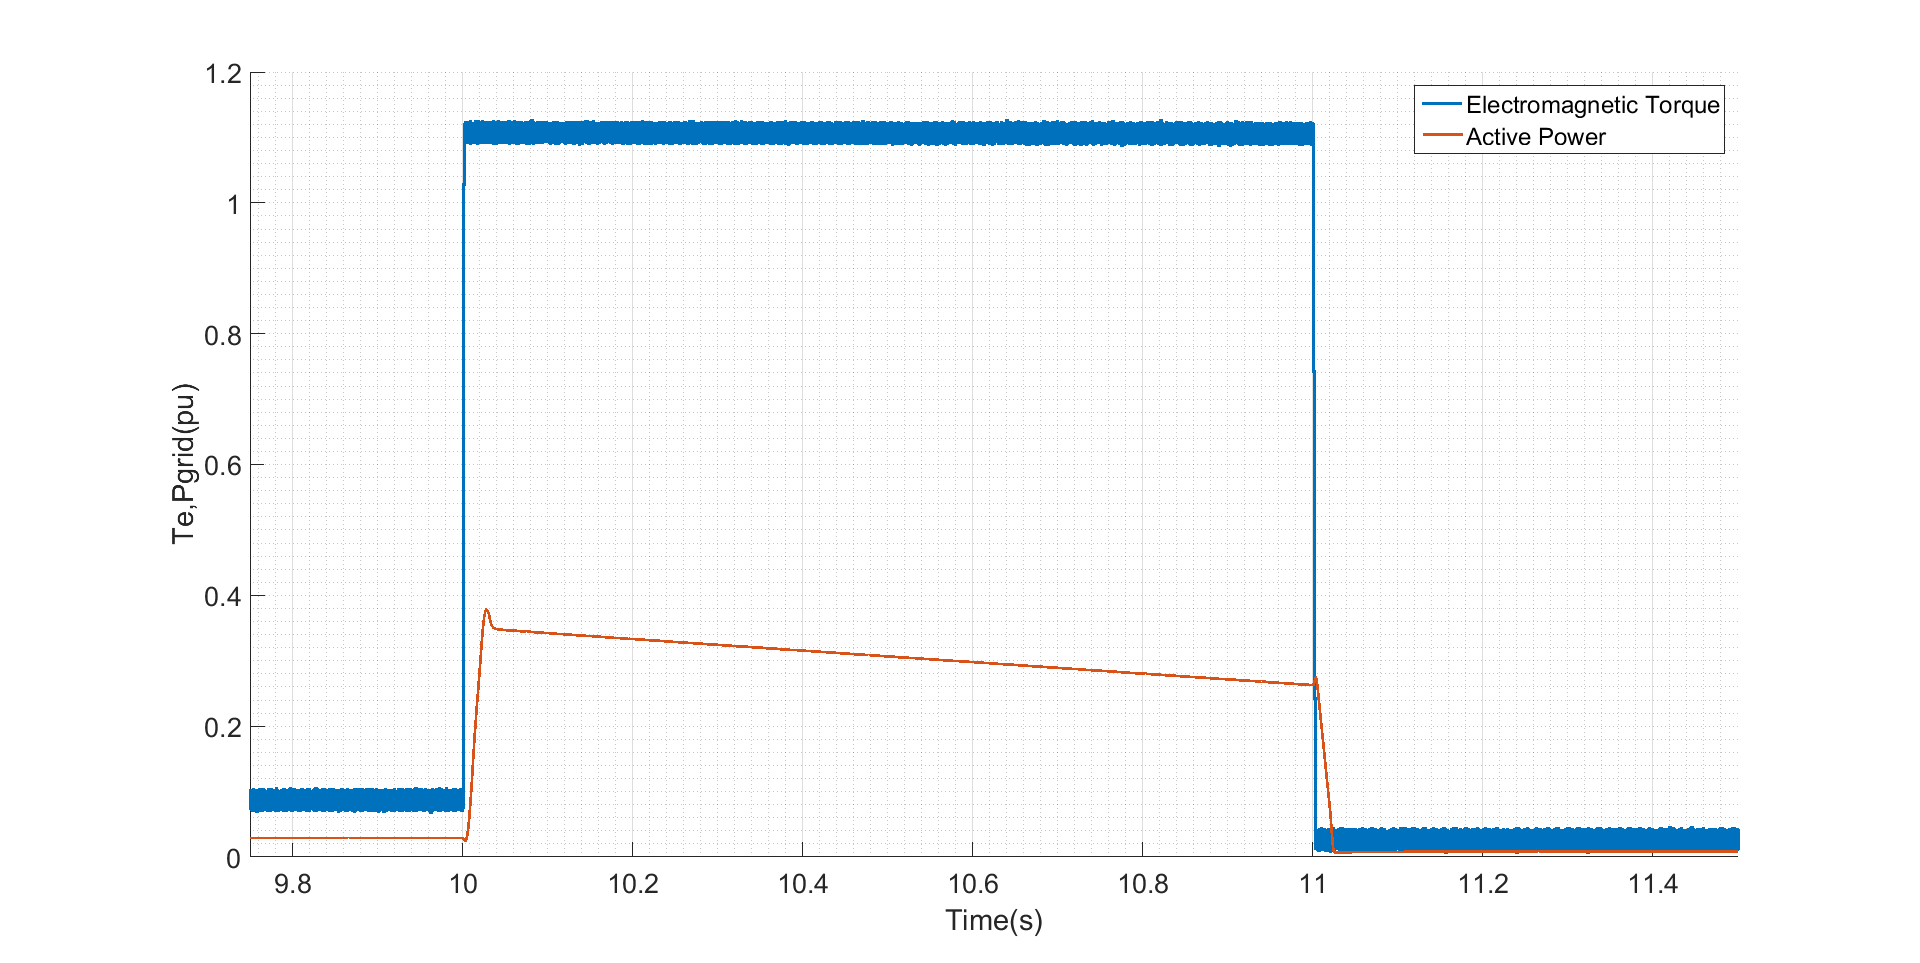
\includegraphics[width=1\linewidth]{power_torque_low_limit.png}
	\caption{Active Power Output of the Wind Turbine for Low Wind Scenario}
	\label{low_limit_power}
\end{figure}
\subsubsection{Active Power in Low Wind Scenario}
The active power of the wind turbine is increased 10\% for three different time intervals as 5, 10 and 20 seconds. The active power output of the wind turbine is given in Fig. \ref{lowactivepowers}. It is observed that turbine power decreases below the nominal value after the support period in order to recover the generator speed. Another observation is the fact that higher support time creates higher dip in the active power in the speed recovery period.\par
\begin{figure}[h!]
	\centering
	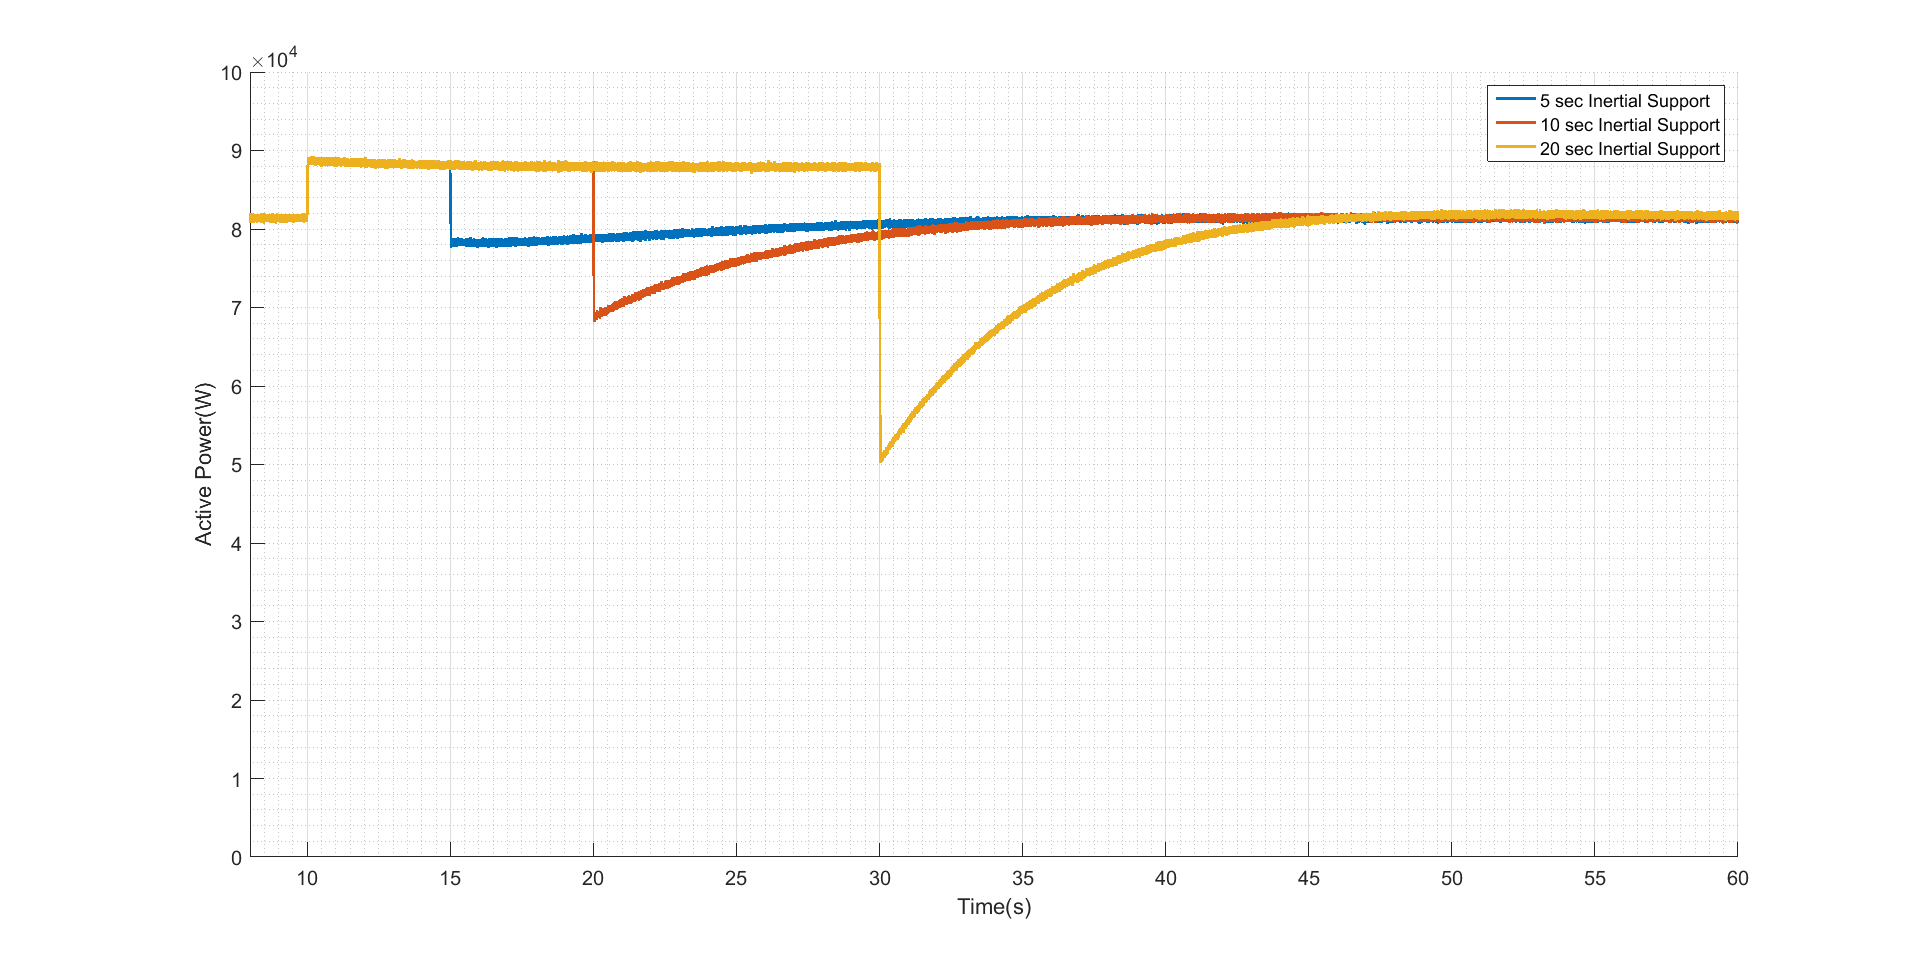
\includegraphics[width=.9\linewidth]{lowwindpowers.png}
	\caption{Active Power Output of the Wind Turbine for Low Wind Scenario}
	\label{lowactivepowers}
\end{figure}
The source of the increased active power in this study is the kinetic energy in the turbine inertia. Therefore, additional active power is extracted from this energy causing a decrease in the wind turbine generator. Generator speed decreases continuously until the support is ended. The generator speeds are shown in Fig. \ref{low_speeds} for three support times.\par
\begin{figure}[h!]
	\centering
	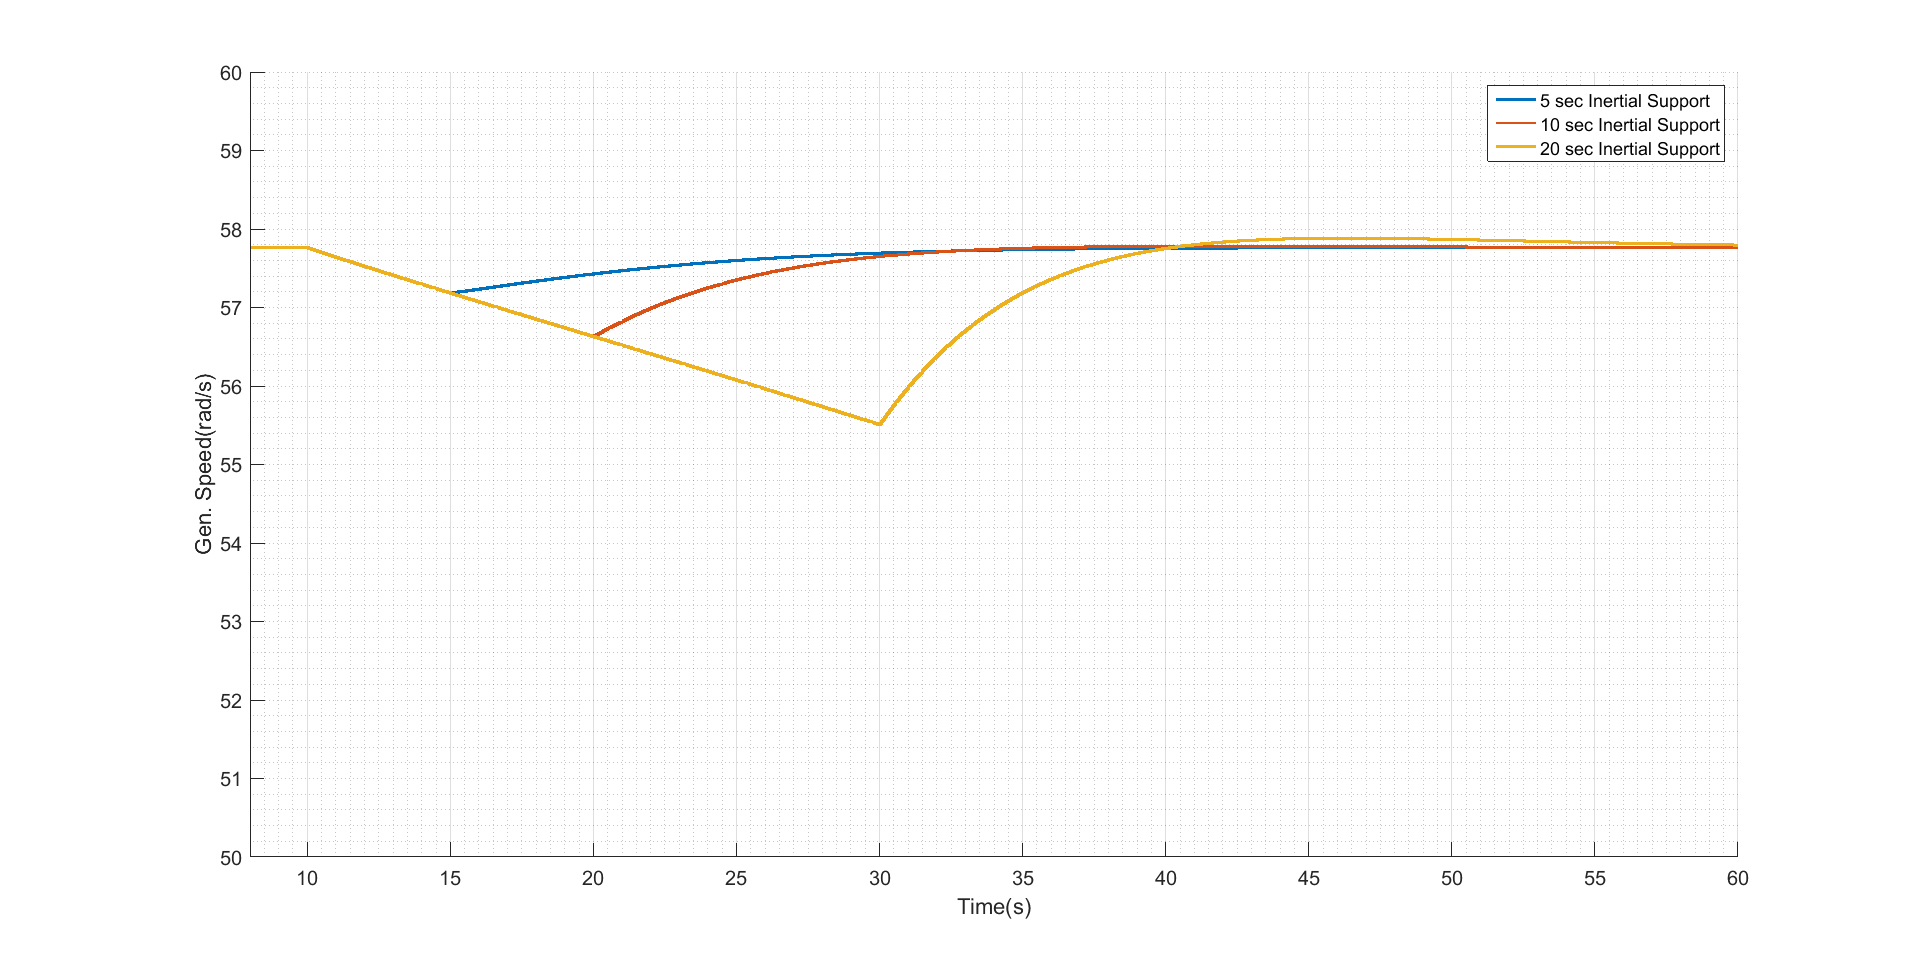
\includegraphics[width=1.0\linewidth]{lowspeeds.png}
	\caption{Generator Speeds of the Wind Turbine for Low Wind Scenario}
	\label{low_speeds}
\end{figure}
The decrease in the generator speed is obtained with an increase in the generator torque. The turbine torque, generator torque and generator speed for 5 seconds support is given in Fig. \ref{low_torques}. The generator torque is increased at t=10s for a time duration of 5 seconds. Turbine torque increases slightly with decreasing speed. However, the increase in the turbine torque is negligible when it is compared to the increase in generator torque as shown in zoomed graph. Therefore, the turbine torque is assumed to be constant for the support period. Turbine and generator torques for the 10 and 20 seconds cases are also shown in Fig. \ref{low_torques2} and Fig. \ref{low_torques3}. 
\begin{figure}[h!]
	\centering
	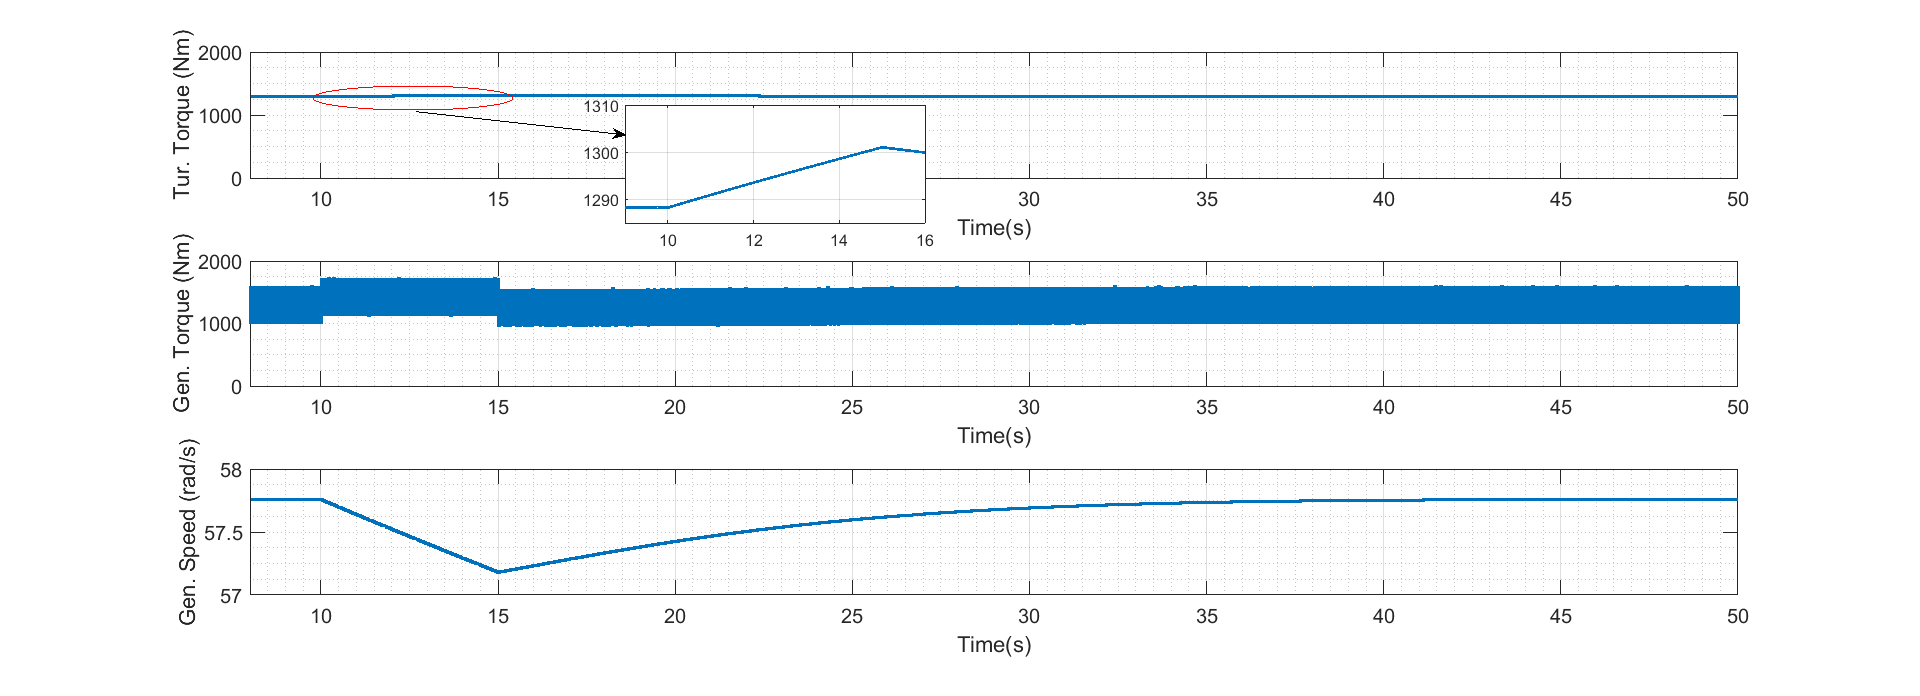
\includegraphics[width=1.0\linewidth]{low_s5_zoomed.png}
	\caption{Turbine Torque, Generator Speed and Torque for 5 Seconds Support under Low Wind Speed}
	\label{low_torques}
\end{figure}
\begin{figure}[h!]
	\centering
	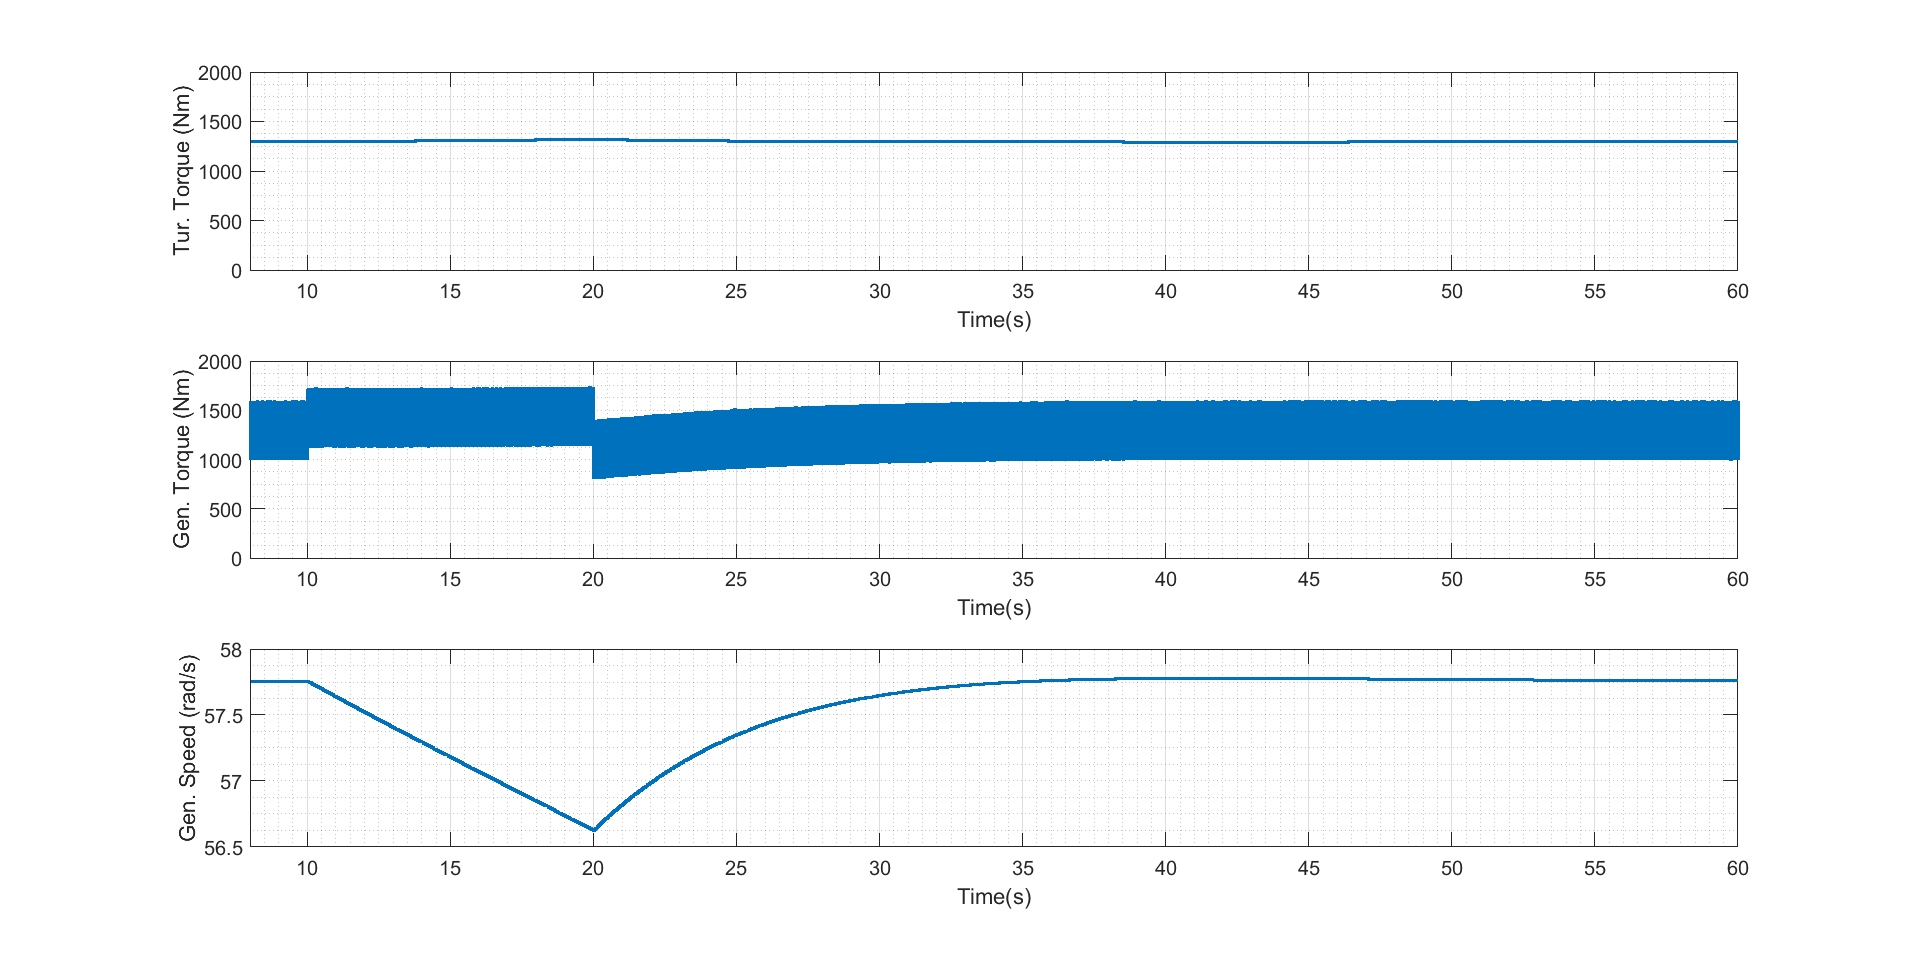
\includegraphics[width=1.0\linewidth]{low_s10.png}
	\caption{Turbine Torque, Generator Speed and Torque for 10 Seconds Support under Low Wind Speed}
	\label{low_torques2}
\end{figure}
\begin{figure}[h!]
	\centering
	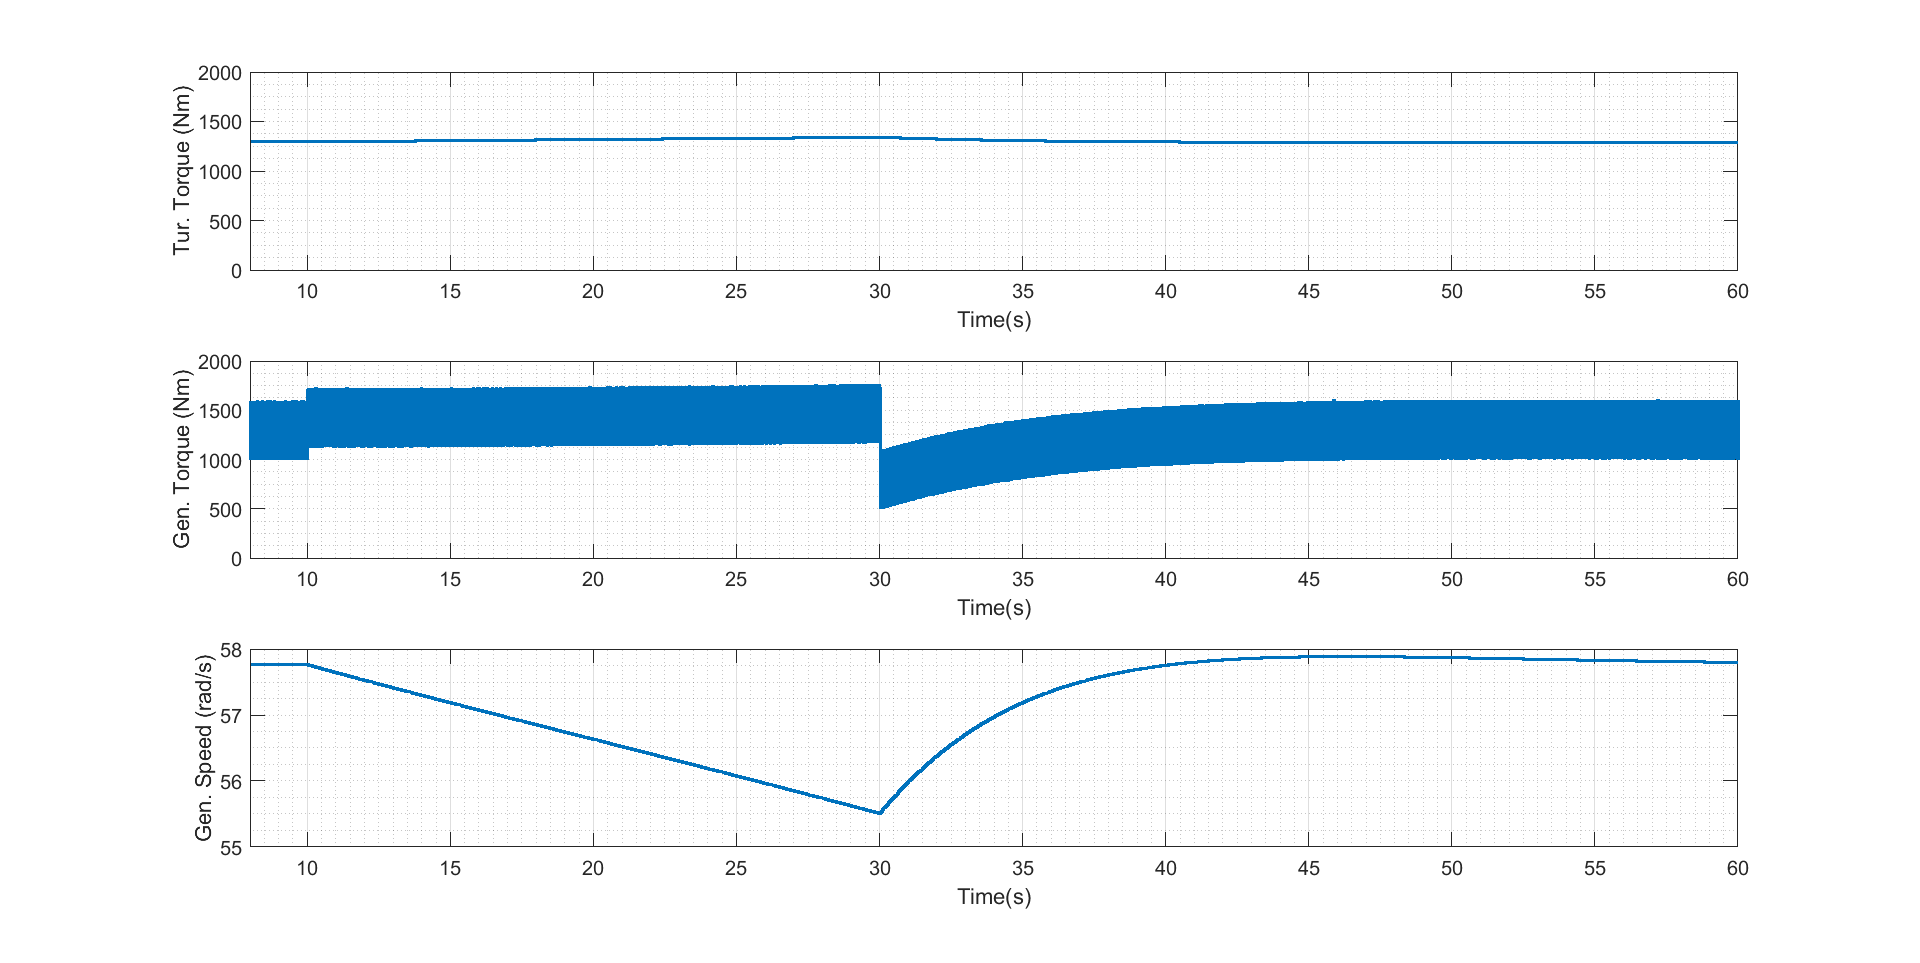
\includegraphics[width=1.0\linewidth]{low_s20.png}
	\caption{Turbine Torque, Generator Speed and Torque for 20 Seconds Support under Low Wind Speed}
	\label{low_torques3}
\end{figure}
Another important criteria on inertial support studies is the DC-Link voltage. When the active power is increased, increased amount of active power is transferred from MSC to GSC. Increased active power should be injected to grid without causing excessive voltage rise on the DC-bus. Note that the voltage rise in the very first seconds in inertial support activation is same for all three support cases. However, the voltage drop will be highest in the 20 seconds case. DC-link voltage for 20 seconds support case is given in Fig. \ref{low_vdc_s20}. The rise on DC-bus voltage can be considered as negligible meanwhile the voltage drops to 0.9995 pu in 20 seconds support case.
\begin{figure}[h!]
	\centering
	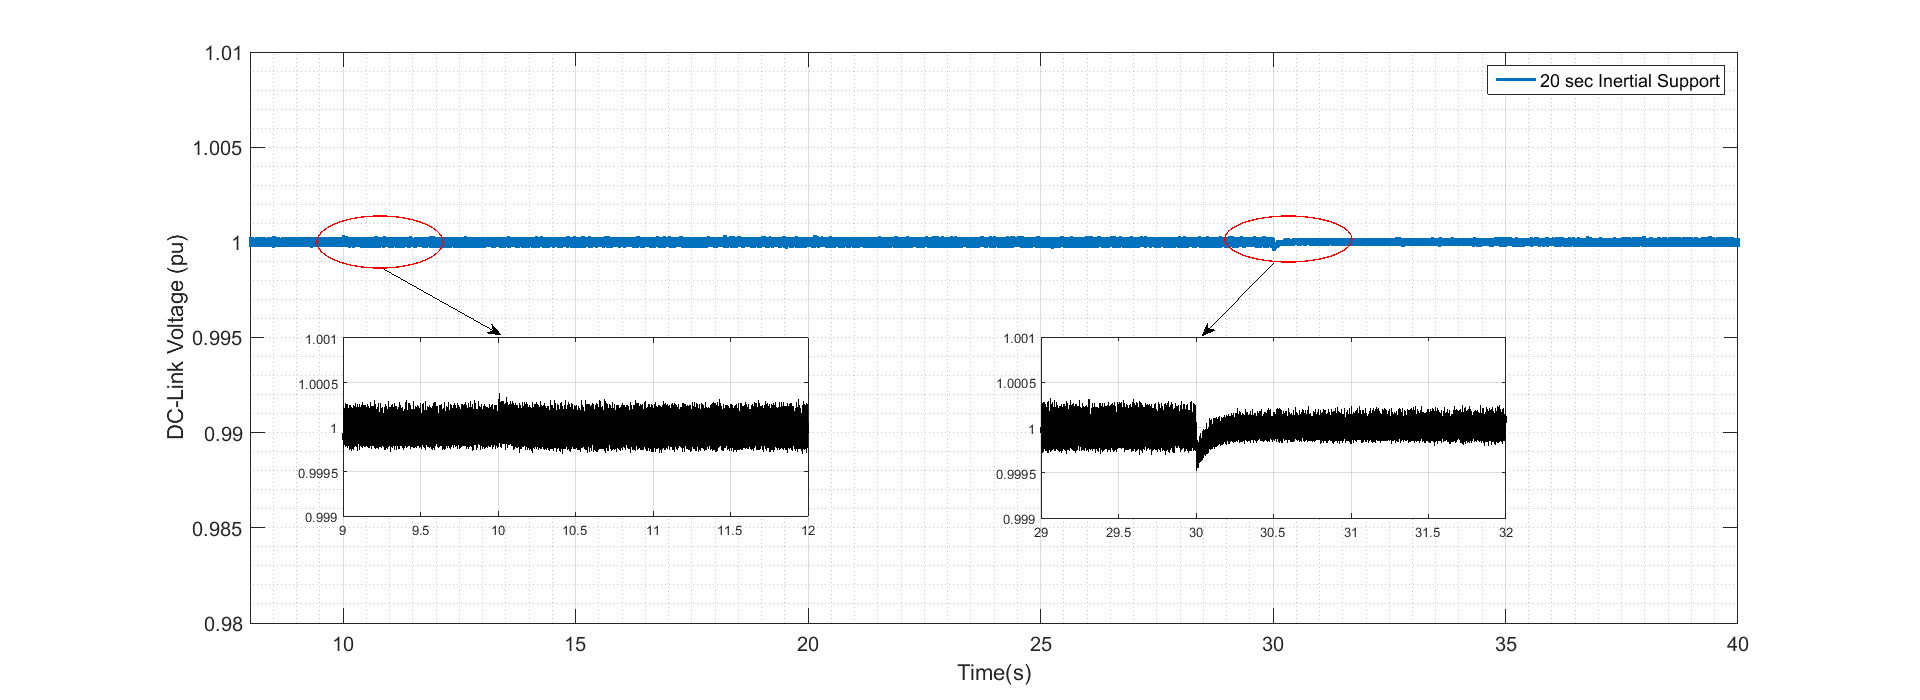
\includegraphics[width=1.0\linewidth]{low_vdc_20.png}
	\caption{DC-Link Voltage for 20 Seconds Support in Low Wind Speed}
	\label{low_vdc_s20}
\end{figure}
\subsection{Medium Wind Scenario}
In the medium wind scenario, wind turbine operated in the middle of the generator speed range. The wind speed is selected as 6m/s in this scenario. 
\subsubsection{Active Power in Medium Wind Scenario}
The active power of the wind turbine is increased by 10\% to provide an inertial support and it is shown in Fig. \ref{midpowers}. The recovery period of shortest support case is much more smoother than the longer ones. When the support time is increased, active power of the wind turbine is almost halved that might cause also problems in frequency stability of the power systems.
\begin{figure}[h!]
	\centering
	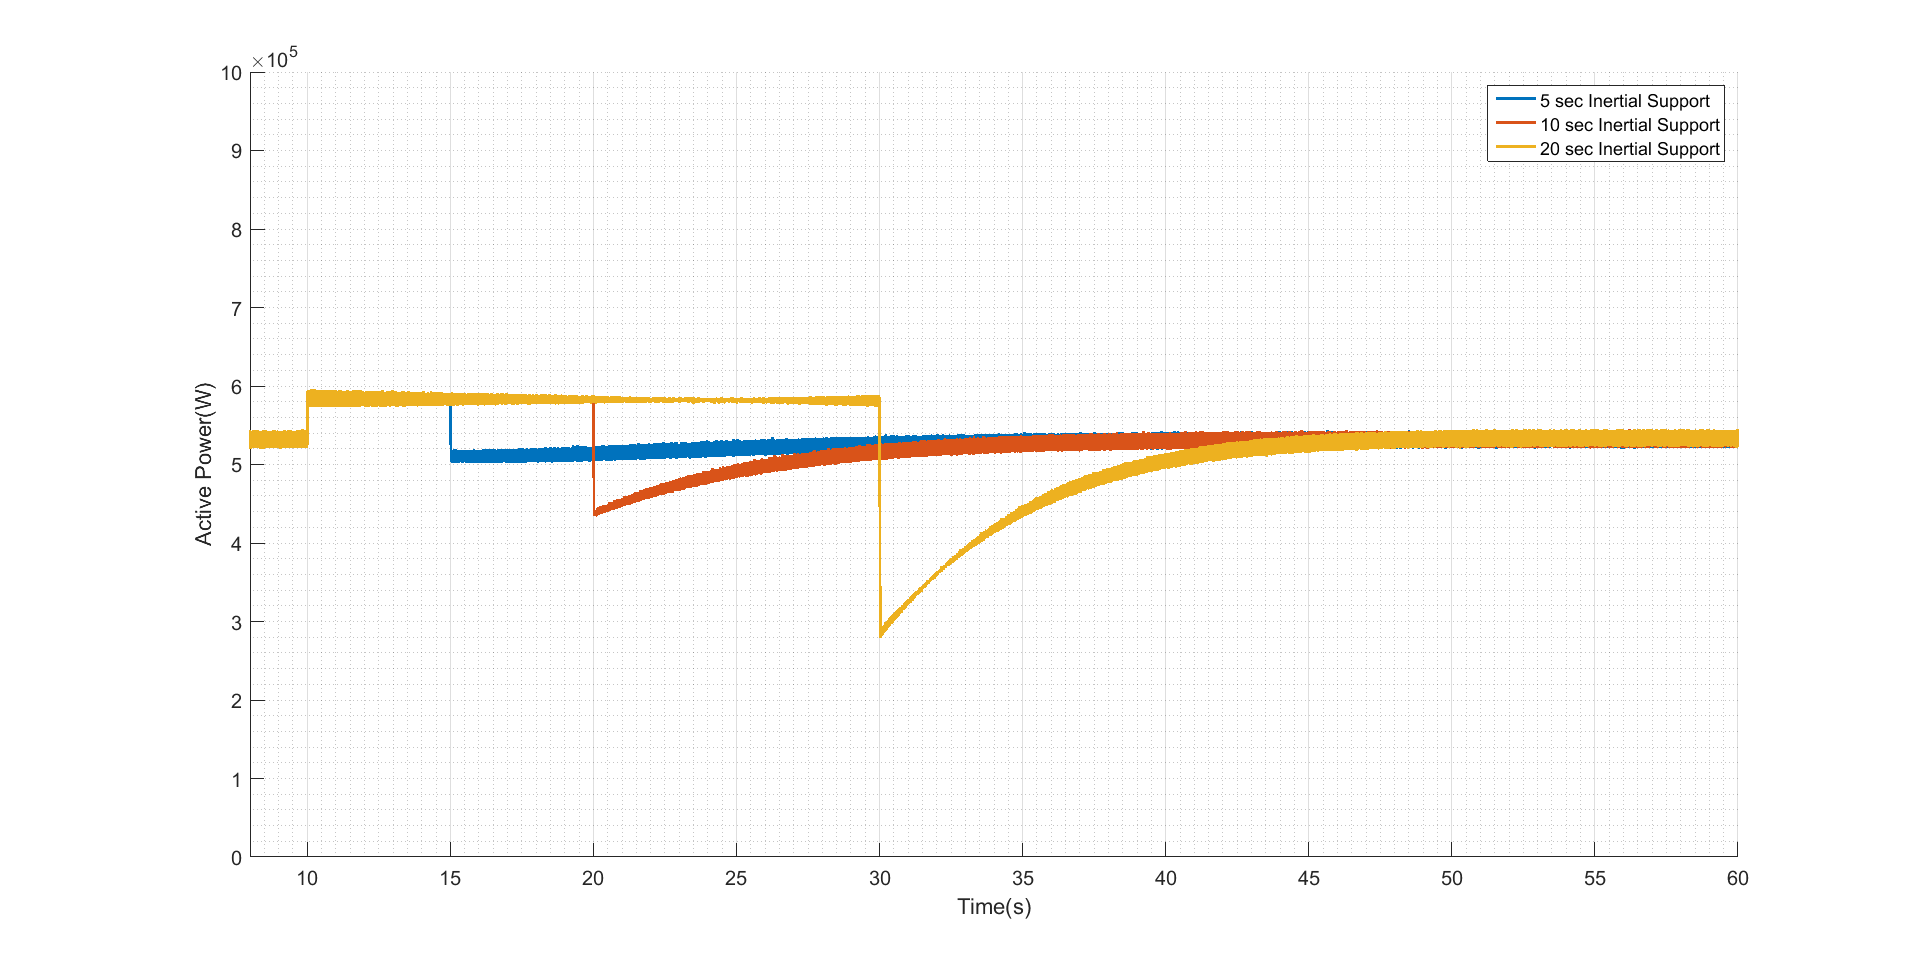
\includegraphics[width=1.0\linewidth]{medium_powers.png}
	\caption{Active Power Output of the Wind Turbine for Medium Wind Scenario}
	\label{midpowers}
\end{figure}
\subsubsection{Generator Speed, Turbine and Generator Torques in Medium Wind Scenario}
In medium wind scenario, higher support time causes decreased active power after the support is ended. The reason is the lower speed value obtained with higher support time. Generator torque is decreased much higher for this case in order to recover the speed. \par
The generator speed, turbine and generator torques are shown in Fig. \ref{mid_torques1}, Fig. \ref{mid_torques2} and Fig.\ref{mid_torques3}. This can be better observed in Fig.\ref{mid_torques3} when the support is ended time at 30 seconds. The negative jump in generator torque crates a negative jump in the active power of the wind turbine since the transferred power is the multiplication of generator torque and generator speed.
\begin{figure}[h!]
	\centering
	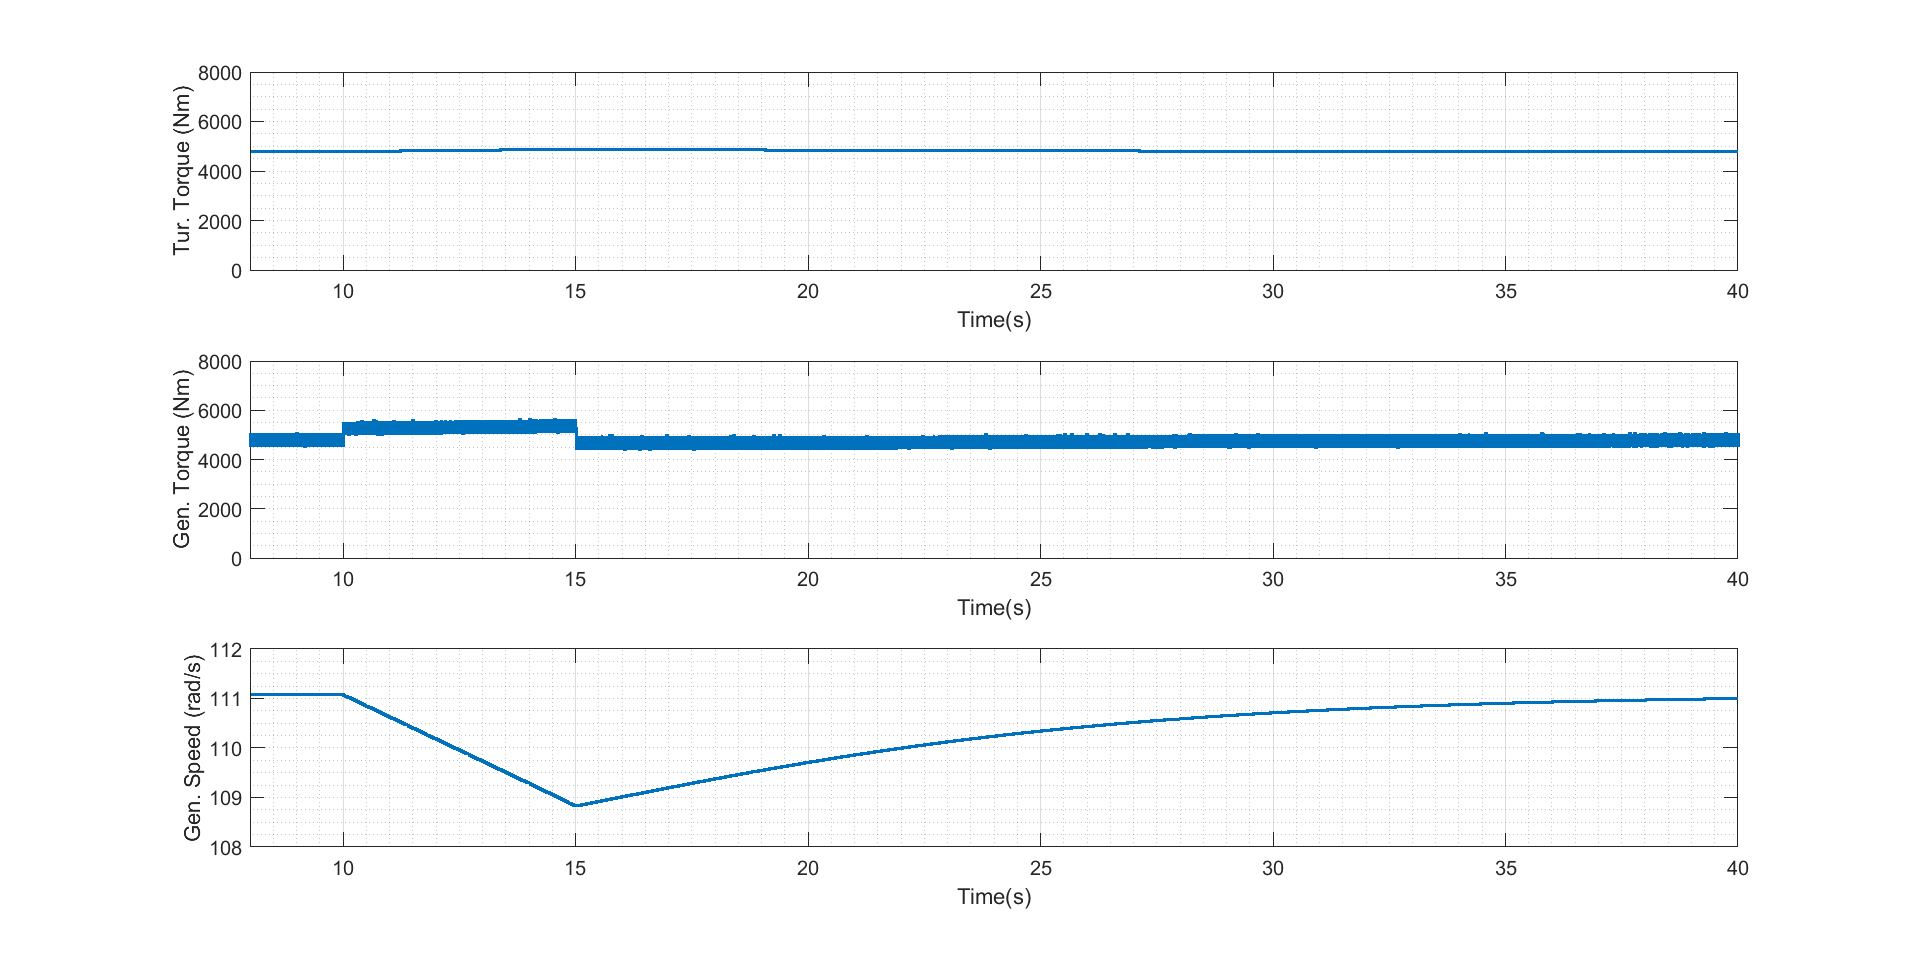
\includegraphics[width=1.0\linewidth]{medium_s5.png}
	\caption{Generator Speed, Generator and Turbine Torques for Medium Wind Scenario for 5 Seconds Support}
	\label{mid_torques1}
\end{figure}
\begin{figure}[h!]
	\centering
	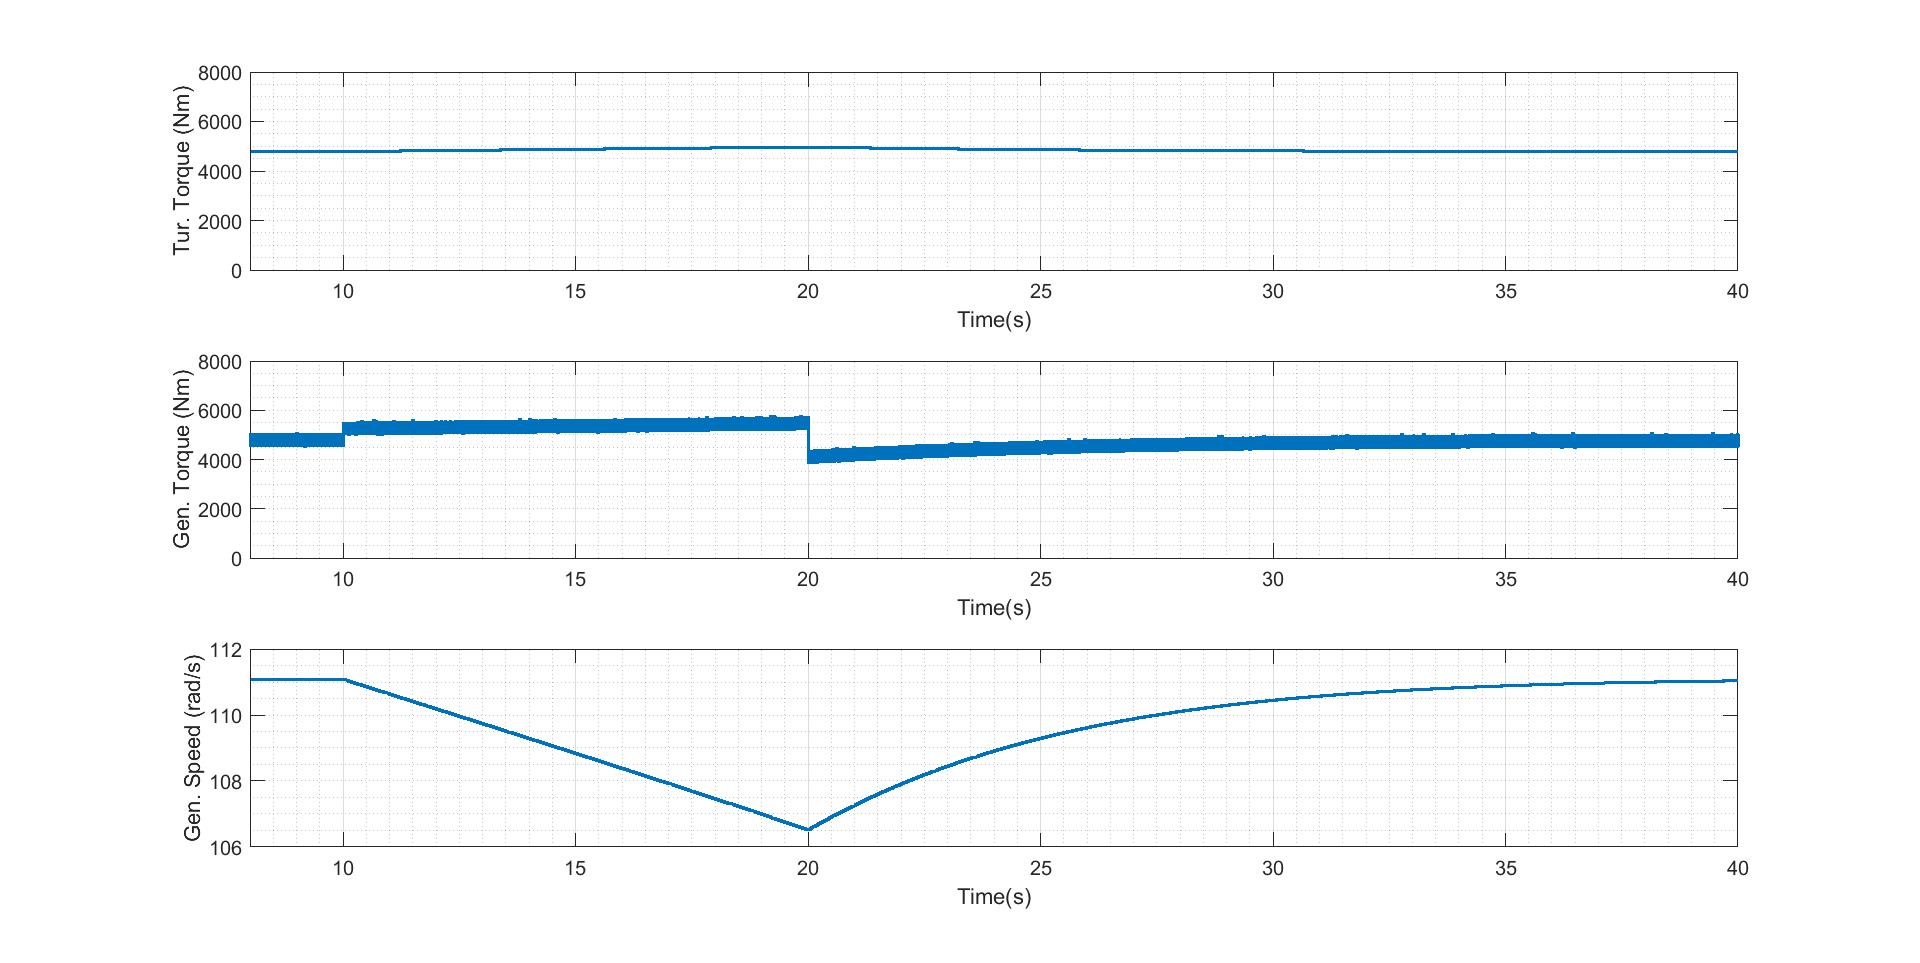
\includegraphics[width=1.0\linewidth]{medium_s10.png}
	\caption{Generator Speed, Generator and Turbine Torques for Medium Wind Scenario for 10 Seconds Support}
	\label{mid_torques2}
\end{figure}
\begin{figure}[h!]
	\centering
	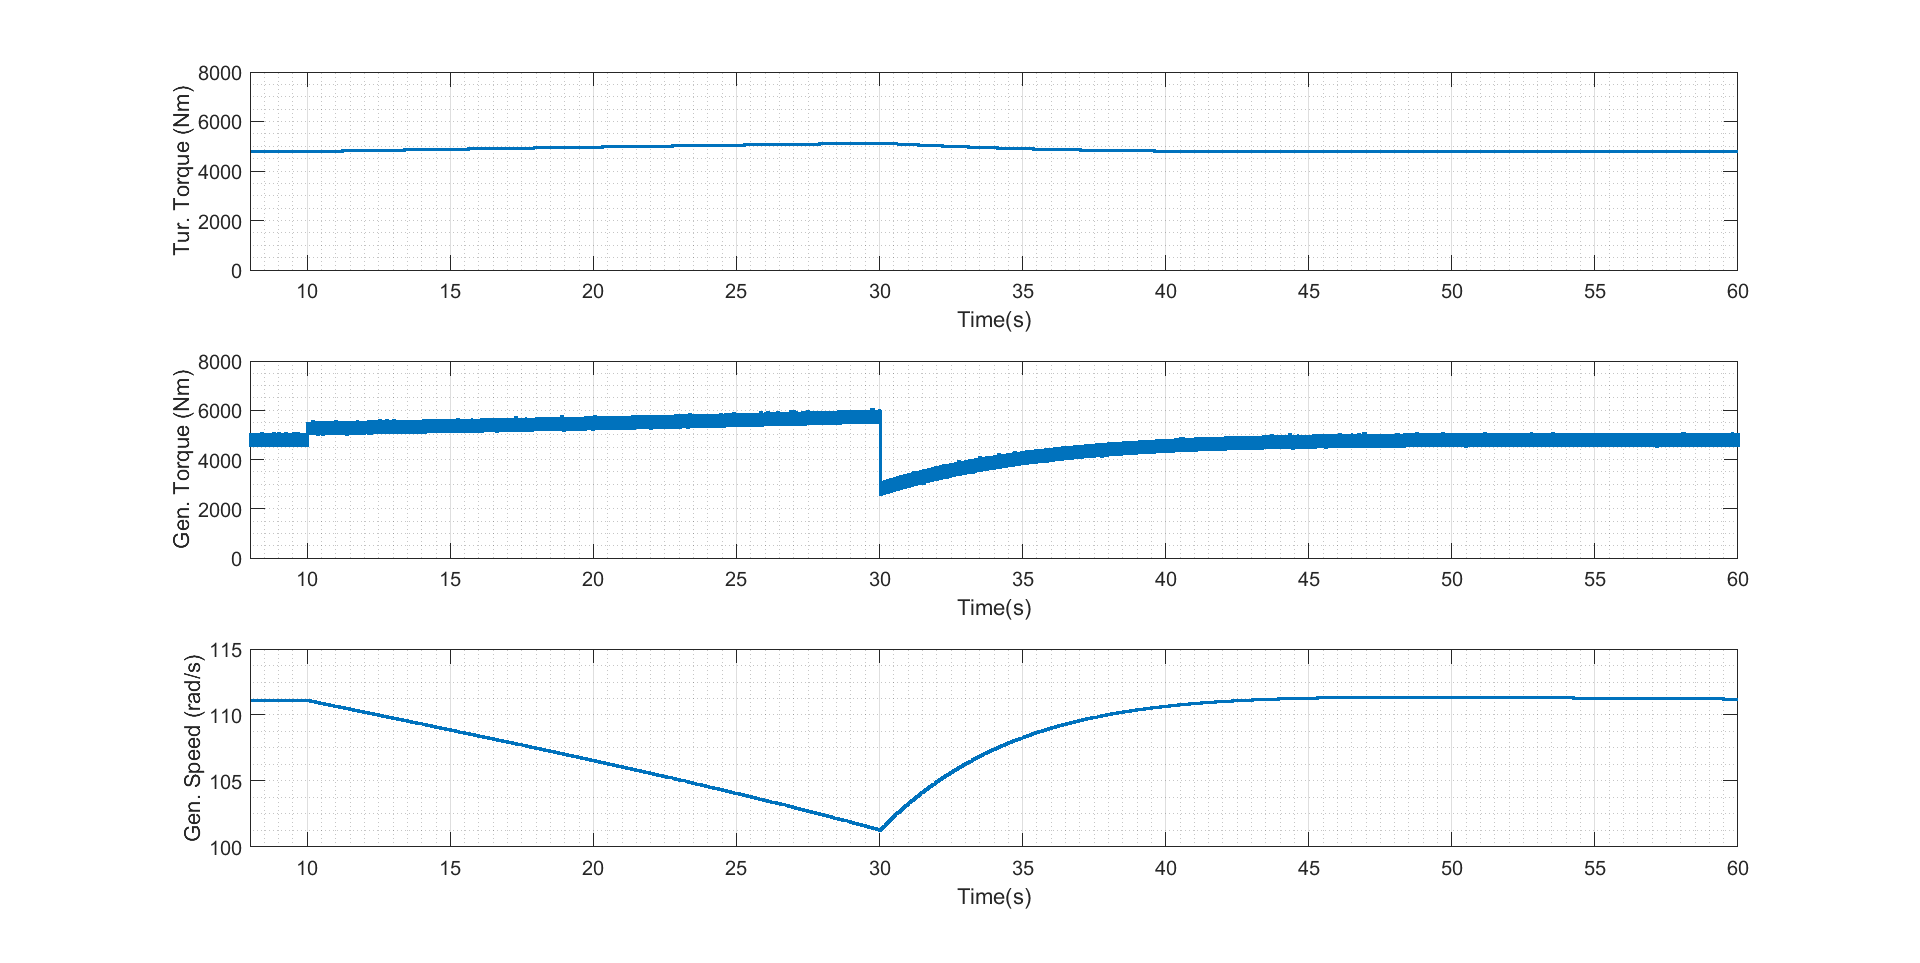
\includegraphics[width=1.0\linewidth]{medium_s20.png}
	\caption{Generator Speed, Generator and Turbine Torques for Medium Wind Scenario for 20 Seconds Support}
	\label{mid_torques3}
\end{figure}
\subsubsection{DC-Link Voltage in Medium Wind Scenario}
The variation of DC-bus voltage with inertial support is shown in Fig. \ref{med_vdc_s20}. The support is activated in time 10 seconds. The rise on the DC-bus voltage is negligible as in the case of low wind scenario. However, the voltage drop at the end of support is much more significant than that of low wind scenario. 
\begin{figure}[h!]
	\centering
	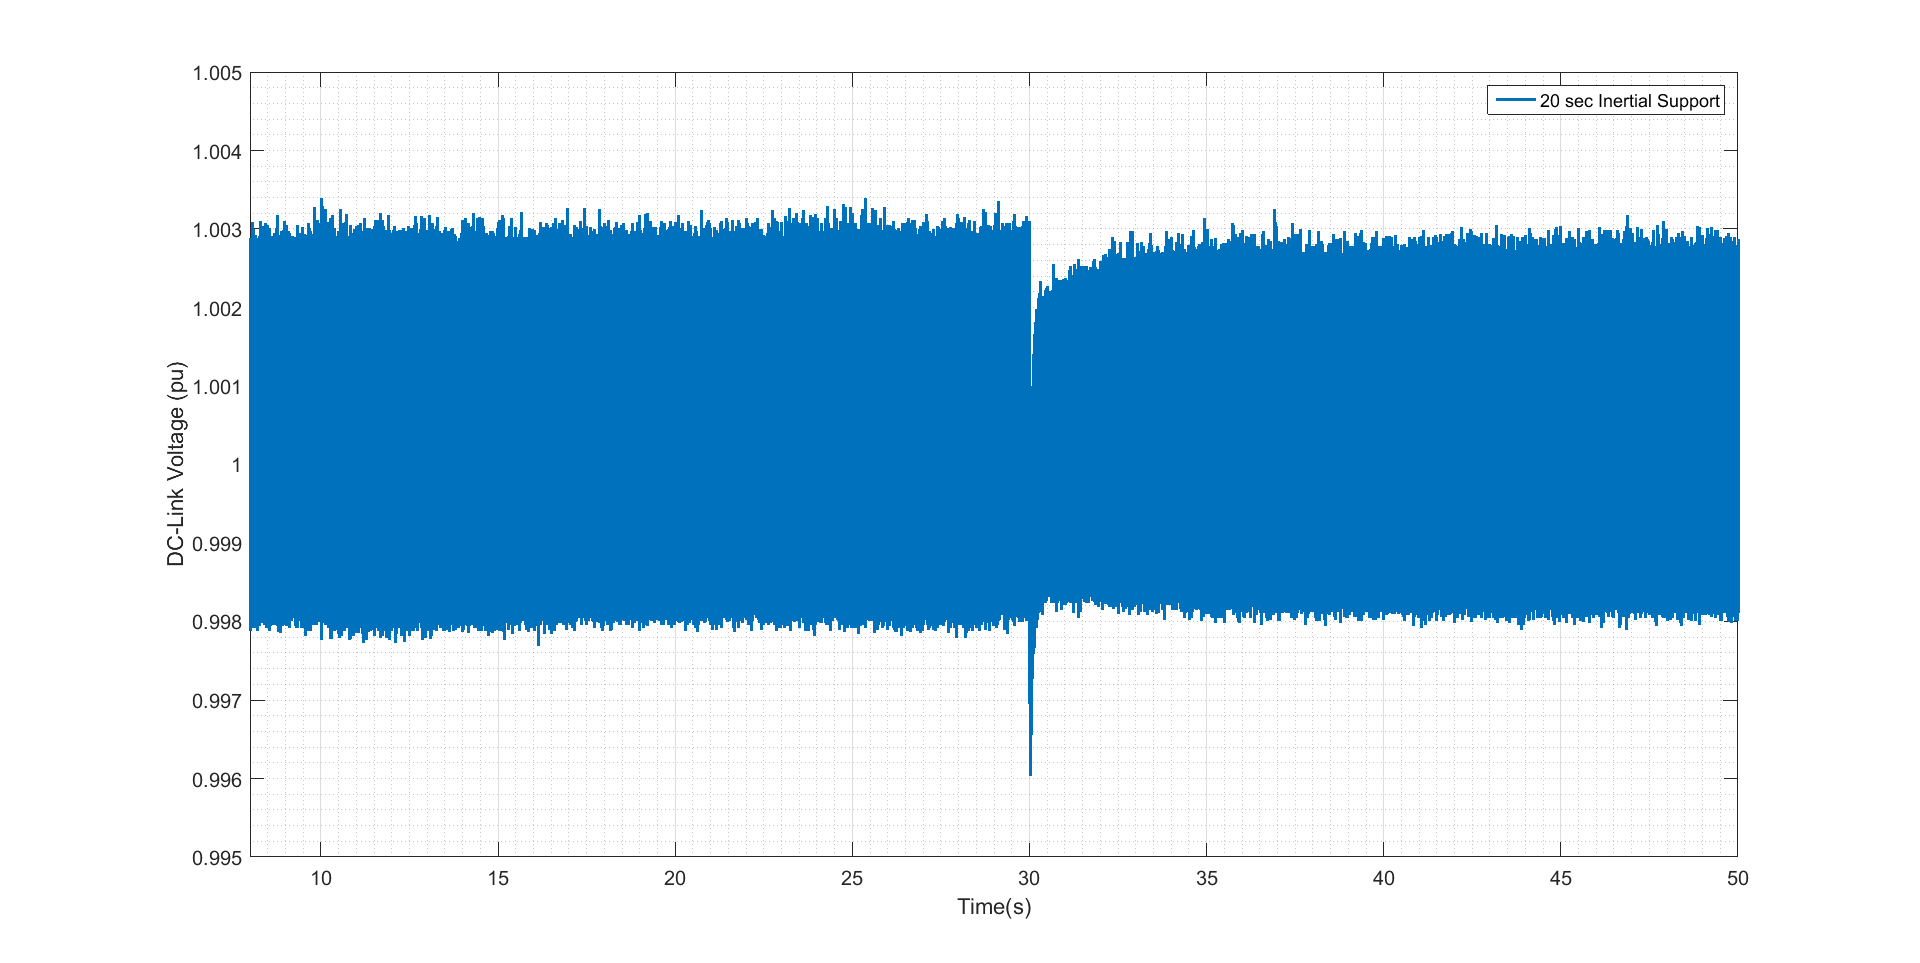
\includegraphics[width=1.0\linewidth]{medium_s20_vdc.png}
	\caption{DC-Link Voltage for 20 Seconds Support in Medium Wind Speed}
	\label{med_vdc_s20}
\end{figure}
\subsection{High Wind Scenario}
In this section, wind turbine operation with high wind speed is investigated. In the high speed operation, the wind turbine injects its maximum power to grid. However, the generator reference speed is the maximum wind speed. Therefore, wind turbine operation is from MPPT operation. Another difference in this section is the pitch angle that curtail wind power and ensure that the generator speed is kept at its maximum. The wind speed in this scenario is selected as 11.4m/s.\par
\subsubsection{Active Power in High Wind Scenario}
Wind turbines are able to provide inertial support in high wind speed as long as converter power rating is higher than the wind turbine power rating. The wind turbine investigated throughout the study has a converter rating of 3.04MVA meanwhile turbine power rating of 2.75MW. Therefore, active power output can be increased up to 3.04MW during support interval. Otherwise, wind turbine cannot provide inertial support for high wind speeds. The active power of the wind turbine is increased by 10\% with three different time intervals. The active powers are shown in Fig. \ref{high_powers}.\par
\begin{figure}[h!]
	\centering
	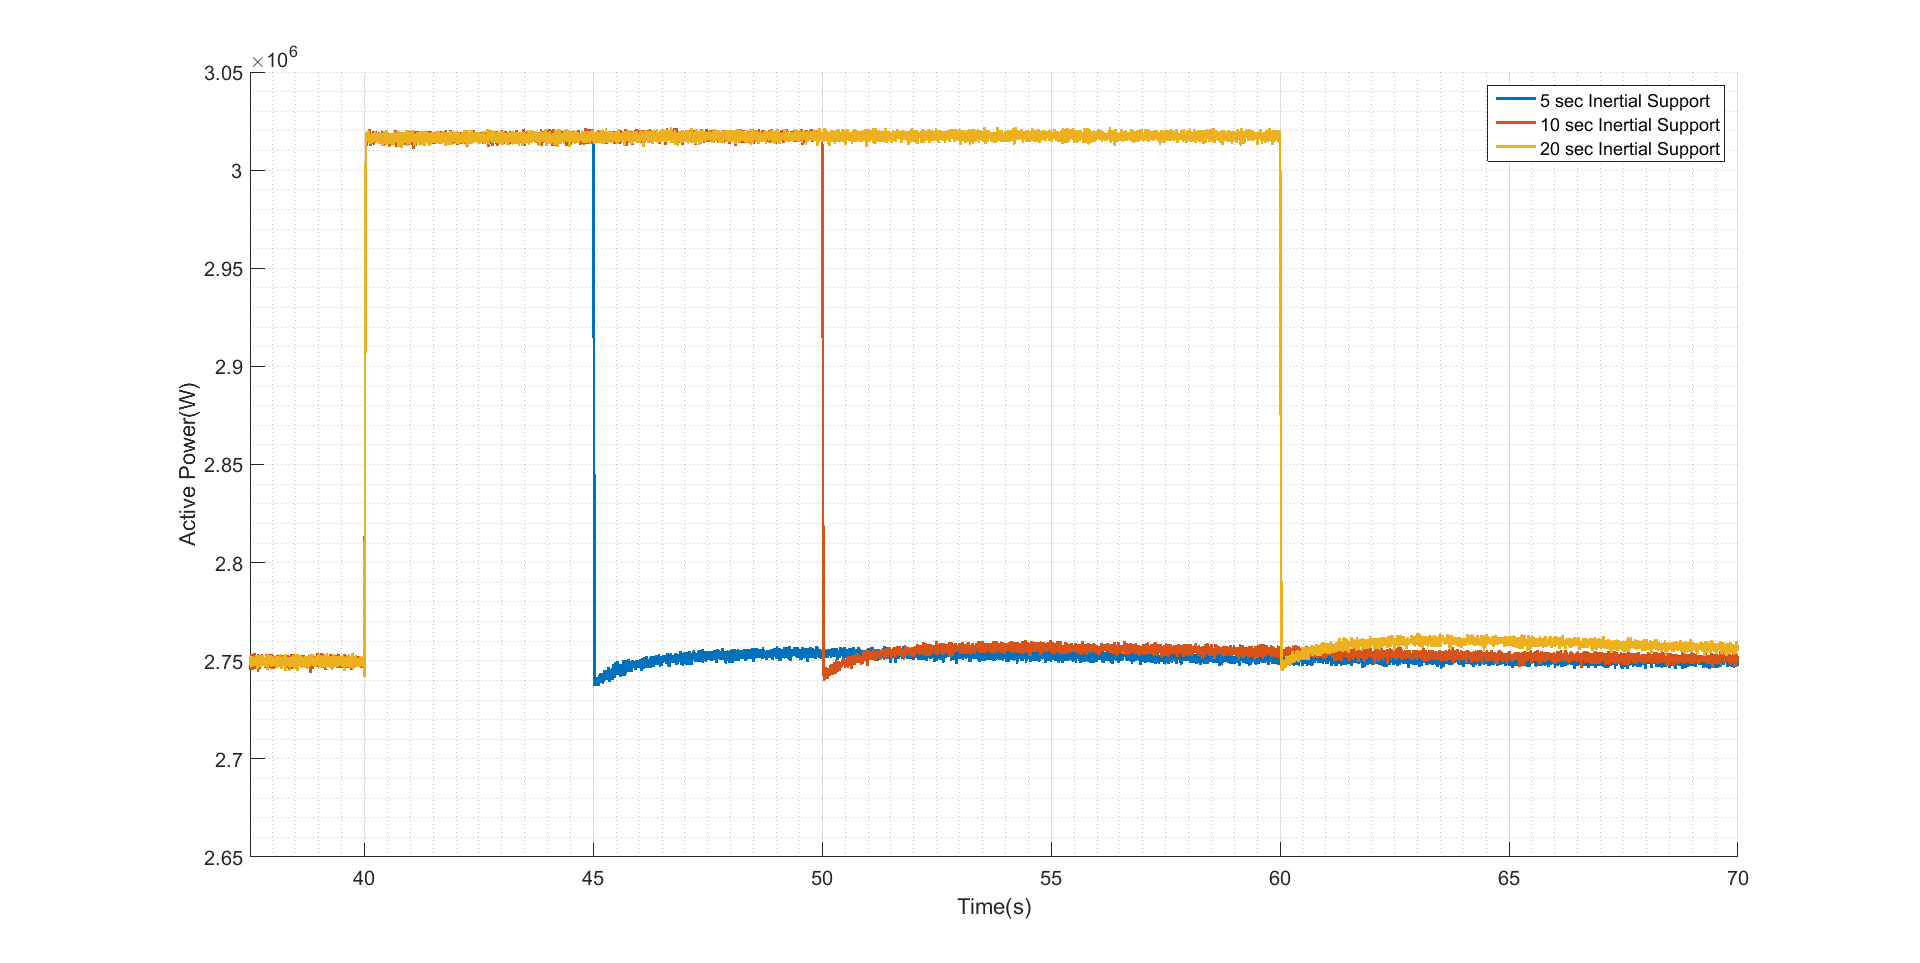
\includegraphics[width=1.0\linewidth]{high_s5_10_20_power.png}
	\caption{Active Power Output of the Wind Turbine for High Wind Scenario}
	\label{high_powers}
\end{figure}
An interesting observation in high wind scenario is that there is no speed recovery process. As soon as the speed is decreased, the pitch controller decreases the blade angle which causes an increase in turbine torque. Therefore, in this case, turbine power decreases back to normal rather than a lower power value as in the other scenarios.
\subsubsection{Generator Speed, Turbine and Generator Torques in High Wind Scenario}
In the high wind case, the generator torque hits the limit defined for normal operating conditions. This is why generator speed is regulated with the help of blade angle. Therefore, pitch angle is also important in this section. Generator speed, turbine and generator torques as well as pitch angle for 5, 10 and 20 seconds support cases are shown in Fig. \ref{high_s5}, Fig. \ref{high_s10} and Fig. \ref{high_s20}. Generator speed starts decreasing when the generator torque is increased. However, the pitch controller decreases the blade angle since the generator speed is below the maximum speed. Therefore, the generator speed rises when the pitch angle is decreased. Note that pitch servo acts slower than the generator torque increase time. This is why the generator speed decreases until the pitch angle is decreased. Generator speed might not be disturbed if the pitch controller is able act fast enough.\par
\begin{figure}[h!]
	\centering
	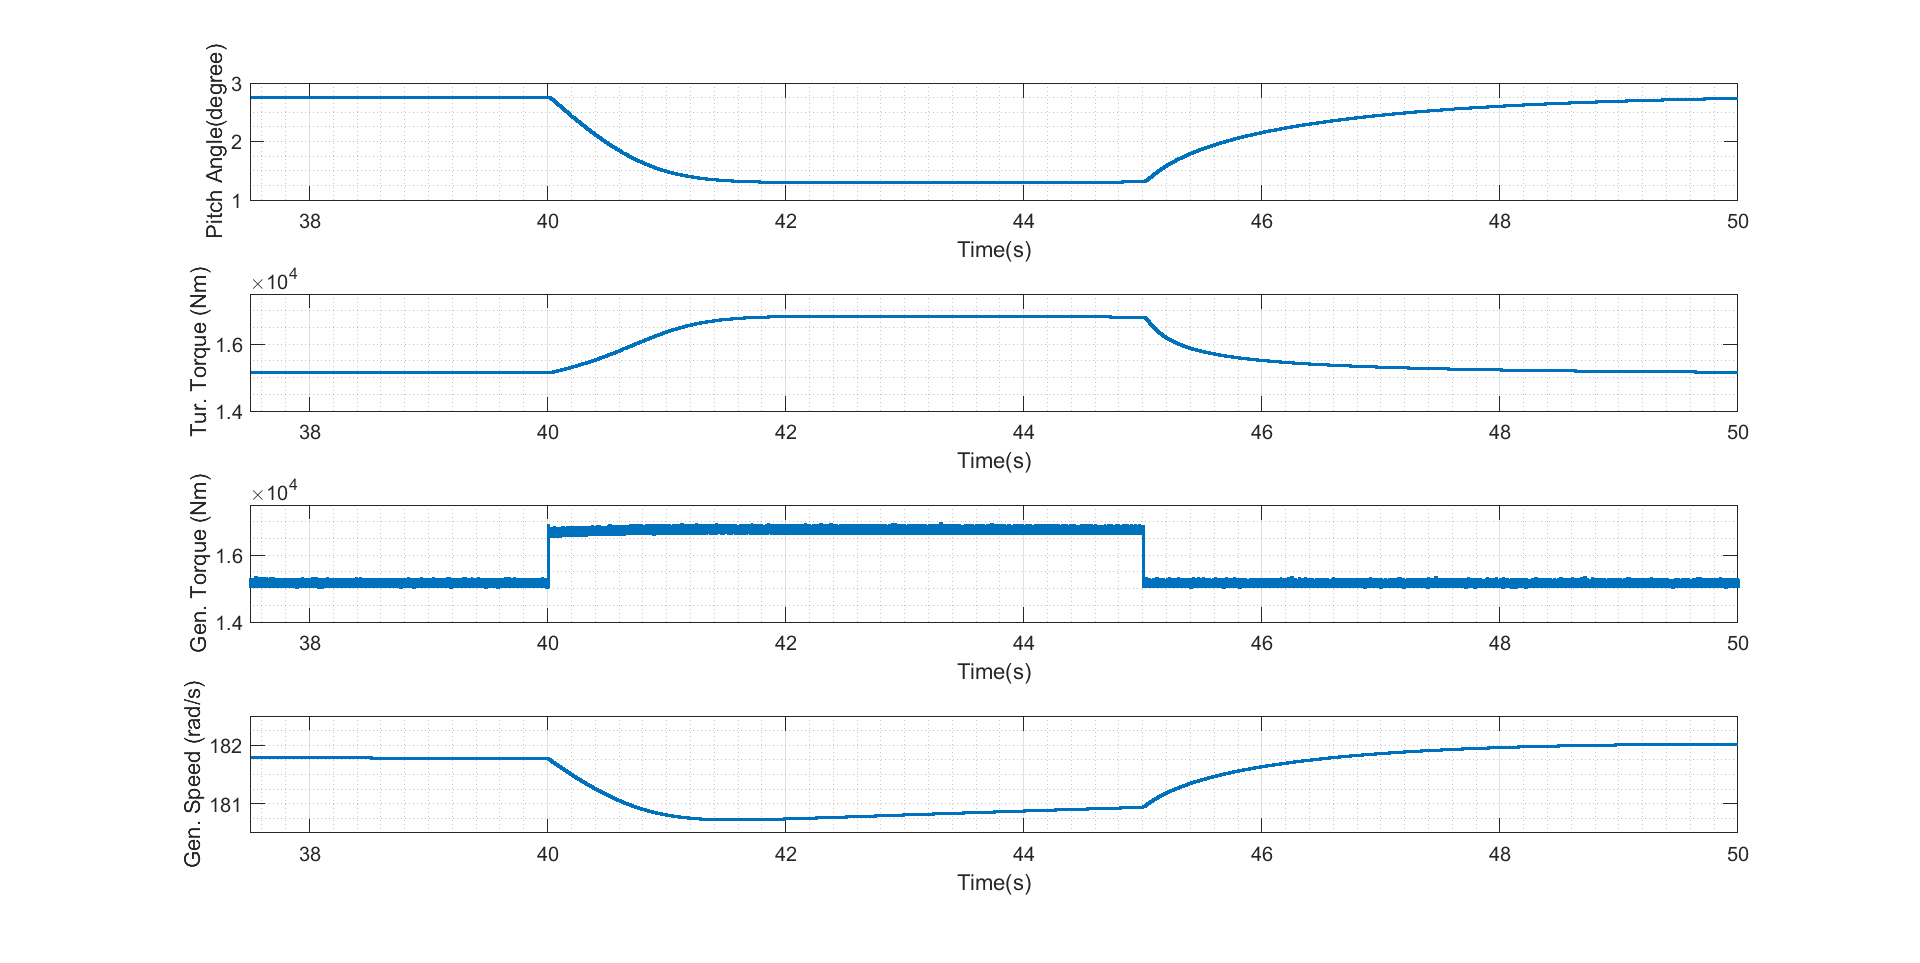
\includegraphics[width=1.0\linewidth]{high_s5_with_torques.png}
	\caption{Pitch Angle, Generator Speed, Generator and Turbine Torques for High Wind Scenario for 5 Seconds Support}
	\label{high_s5}
\end{figure}
\begin{figure}[h!]
	\centering
	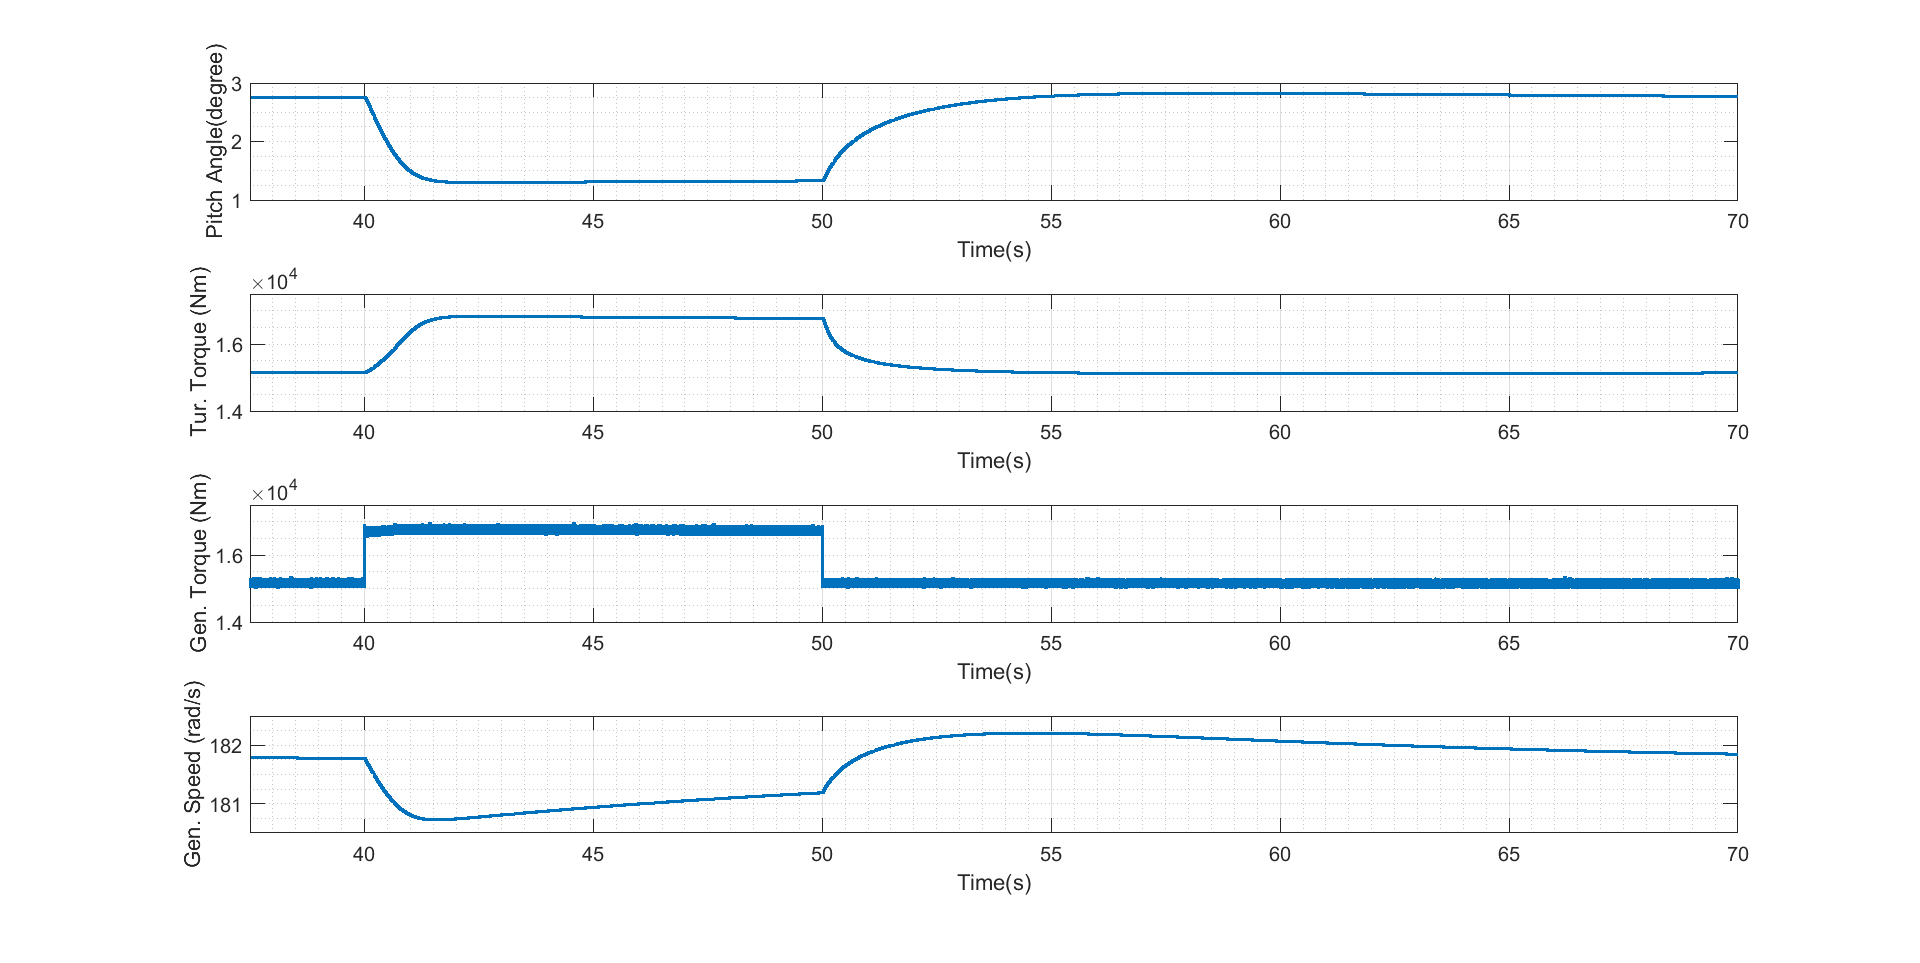
\includegraphics[width=1.0\linewidth]{high_s10_with_torques.png}
	\caption{Pitch Angle, Generator Speed, Generator and Turbine Torques for High Wind Scenario for 10 Seconds Support}
	\label{high_s10}
\end{figure}
\begin{figure}[h!]
	\centering
	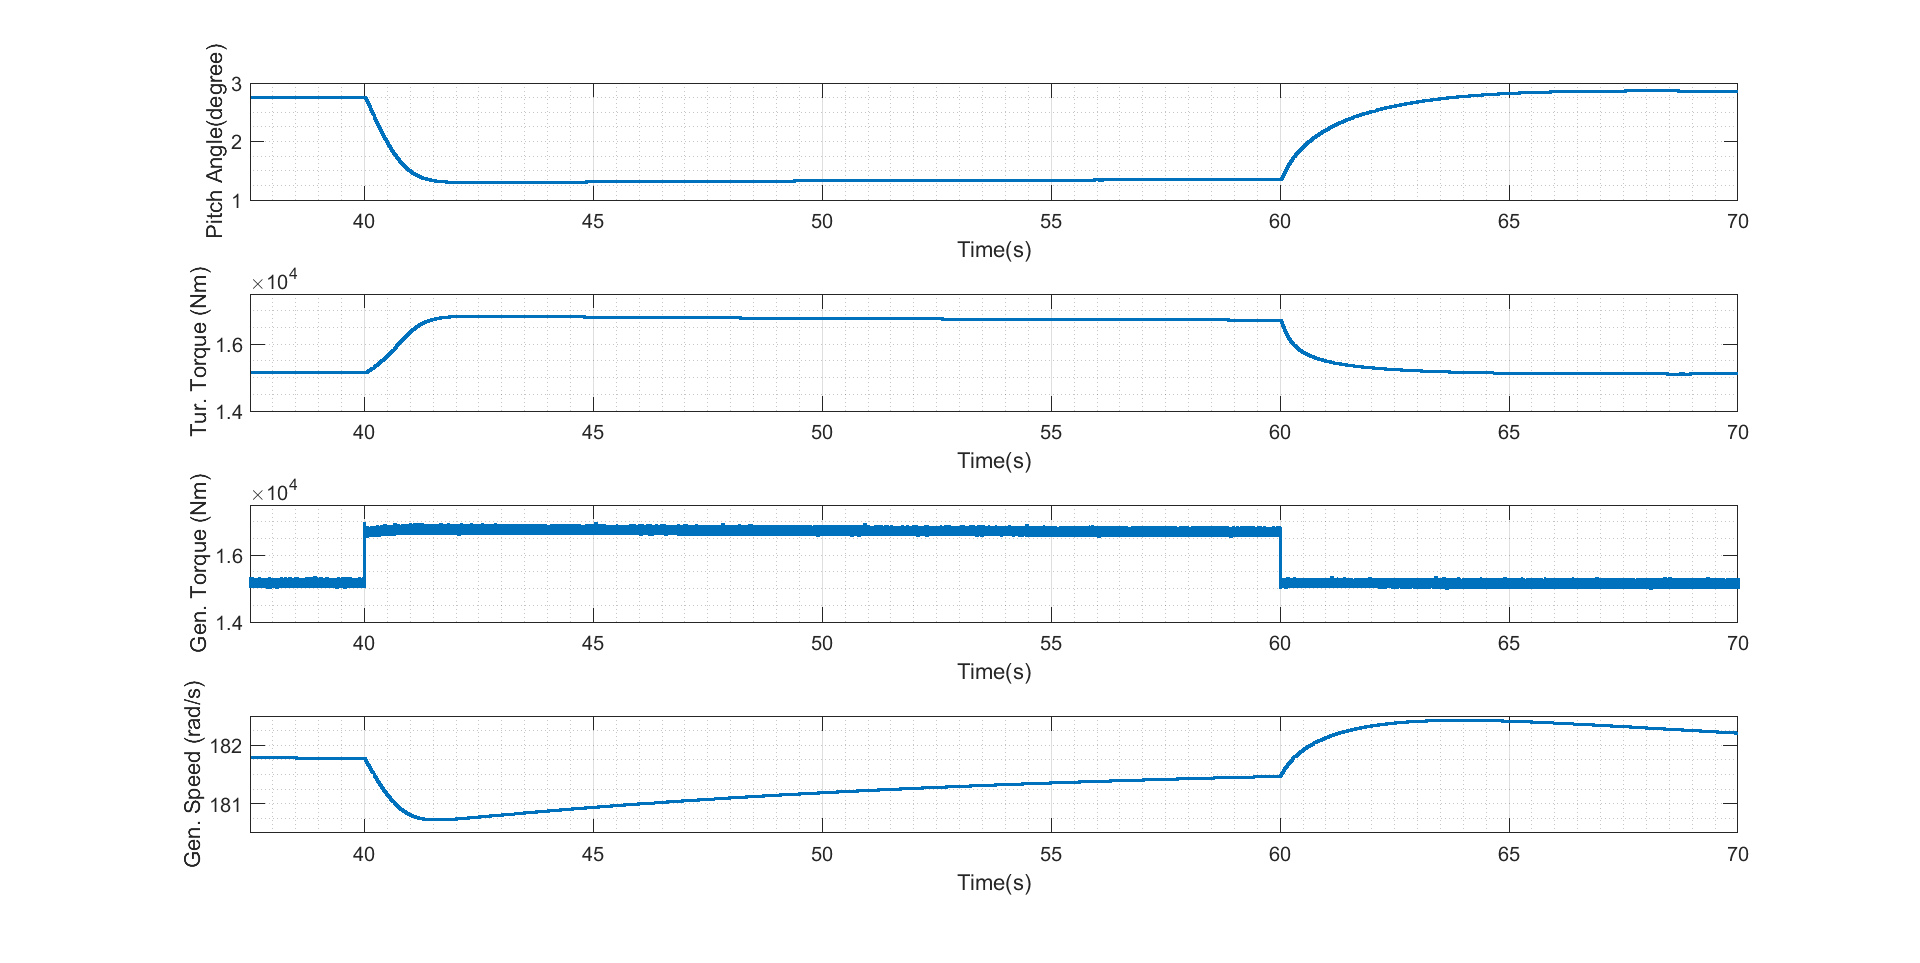
\includegraphics[width=1.0\linewidth]{high_s20_with_torques.png}
	\caption{Pitch Angle, Generator Speed, Generator and Turbine Torques for High Wind Scenario for 20 Seconds Support}
	\label{high_s20}
\end{figure}
In high wind scenario, generator speed rises towards the maximum generator speed thanks to the decrease in blade angle. If the support time is increased, the generator speed will reach the maximum speed, and will stay constant with a new pitch angle. 
\subsubsection{DC-Link Voltage in High Wind Scenario}
The DC-bus voltage is not affected from inertial support on low speed scenario. However, the nominal power and additional power in low speed case is much smaller than that of high wind scenario. The effect of inertial support in high wind case is shown in Fig. \ref{high_s20_vdc}. Nonetheless, the DC-bus voltage is between the range of 0.996 and 1.004 pu in high wind scenario. Note that wind turbines encounter such variations in the DC-bus voltage when the wind speed changes during daily operation. 
\begin{figure}[h!]
	\centering
	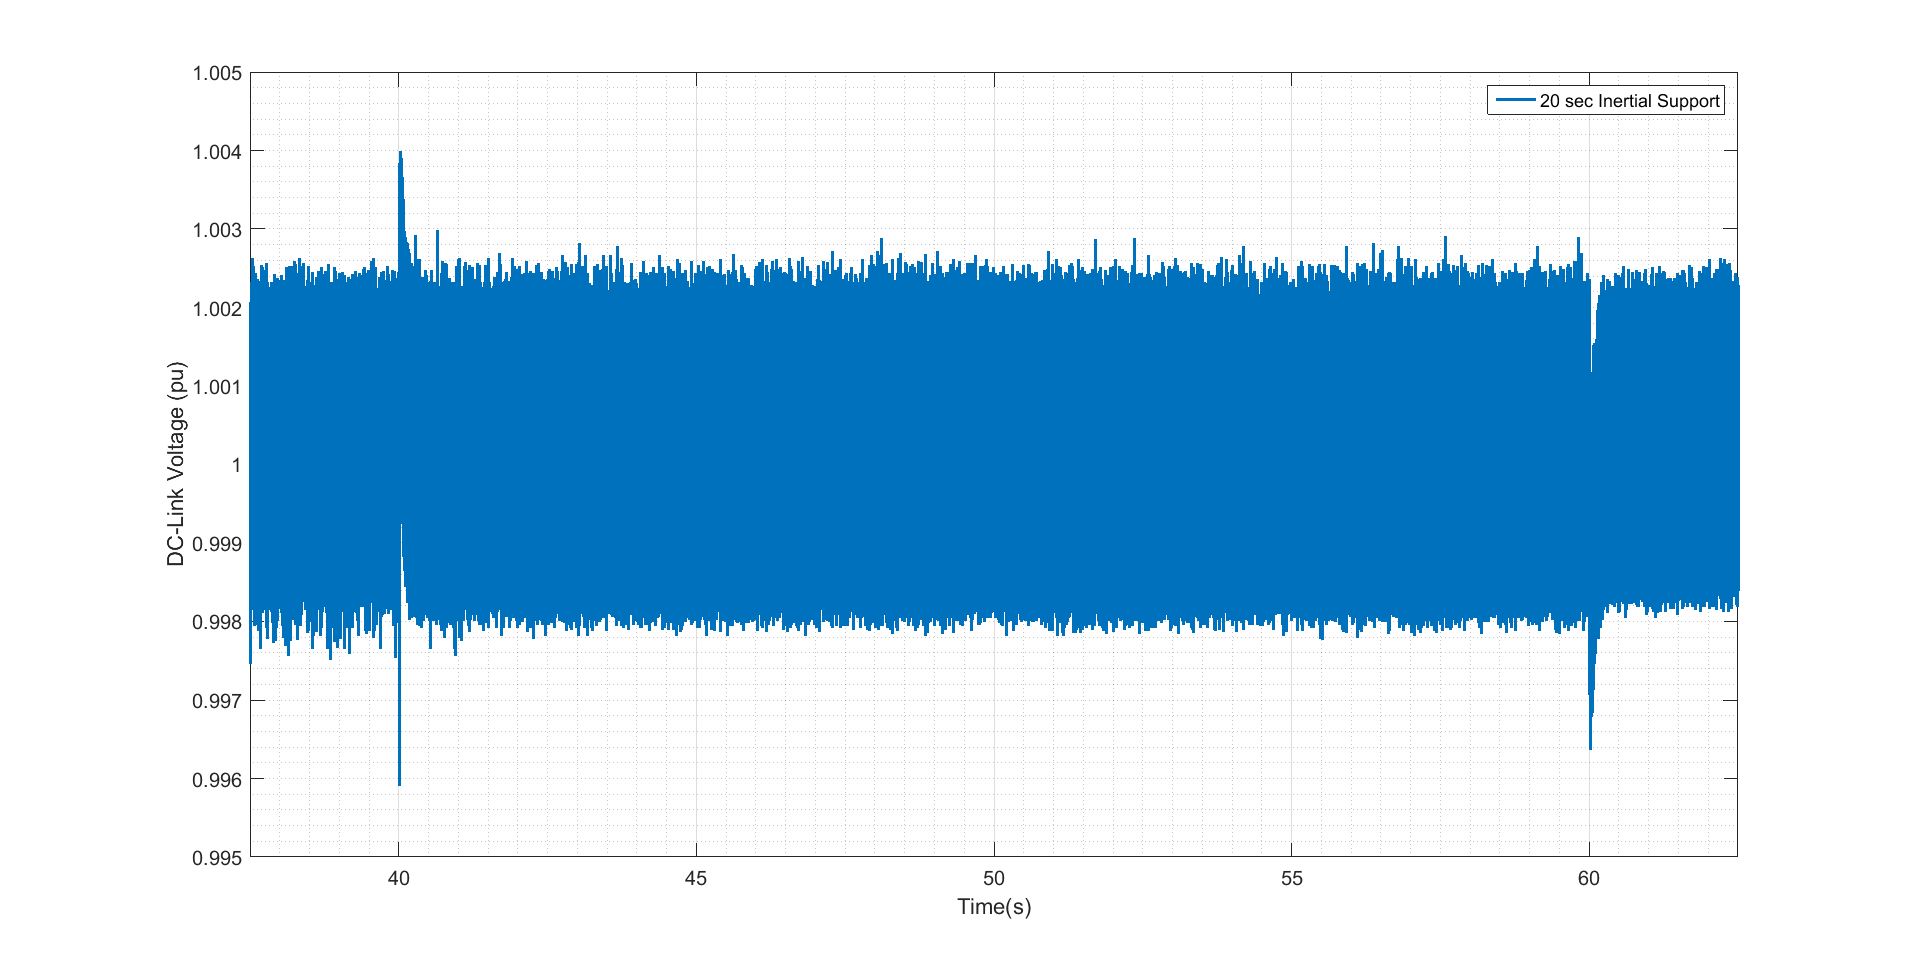
\includegraphics[width=1.0\linewidth]{high_s20_vdc.png}
	\caption{DC-Link Voltage for 20 Seconds Support in High Wind Speed}
	\label{high_s20_vdc}
\end{figure}